\documentclass[a4paper,twoside]{article}
\usepackage{autiwa}
\usepackage{listings}

\title{Débuter avec \LaTeX}

\author{Autiwa}

\makeindex

\begin{document}
\begin{titlepage}

\begin{center}

\vfill
% Upper part of the page
\begin{Huge}\TeX\end{Huge}\hfill
\includegraphics[width=0.15\textwidth]{figure/logo-ubuntu.pdf}\hfill\begin{Huge}\LaTeXe\end{Huge}\\[1cm]

% Title
\HRule \\[0.4cm]
{ \huge \bfseries \makeatletter\@title\makeatother}\\[0.4cm]

\HRule \\[0.75cm]
{\large \today}\\[0.75cm]
\makeatletter
\@author
\makeatother
\vfill
\abstract{Recueil des commandes et astuces que j'ai glané à droite à gauche au fil de mon apprentissage de \LaTeX}
\vfill

% Bottom of the page


\end{center}

\end{titlepage}
\tableofcontents
\newpage

%Stage LaTeX - Niveau Débutant.pdf est bien fait, et complet, notamment pour les tableaux

\section{Généralités}
\subsection{Les Groupes}
Pour écrire a0 au carré en tex, il ne faut pas uniquement mettre le 0 en indice et le 2 en exposant \(a_0^2\), il faut utiliser les groupes pour que le rendu soit joli.

\begin{example}
\[a_0^2\]
\[{a_0}^2\]
\end{example}

\begin{example}
\(\underbrace{\text{expression}}
_\text{commentaire}\)
\end{example}

permet de commenter et de donner des précisions sur une expressions. Je crois que overbrace fait la même chose mais par le haut.

\subsection{Caractères spéciaux et commandes utiles}\index{caractères spéciaux}
\verb|\newpage| affichera les prochains caractères dans une nouvelle page.

\verb|\\| termine une ligne et renvoie à la ligne.

\verb#\verb|commande non exécutée|# : la commande \verb|\verb| permet de ne pas compiler du texte qui sera encadrée par n'importe quel caractère, le premier exemplaire de ce caractère se situant juste après la commande \verb|\verb| et le deuxième juste à la fin.

\begin{example}
\(\backslash\)
\end{example}
mais il faut que ça soit en mode math

\begin{example}
\verb|^| ou encore \(\wedge\)
\end{example}

\begin{example}
100\%
\end{example}

\begin{example}
--- contenu de la parenthese ---
1789--1989
\end{example}

\subsection{Comment faire un paragraphe?}\index{paragraphe}

Une ligne blanche dans le texte crée un saut de paragraphe avec indentation. Tant qu'il n'y a pas de ligne blanche, et même s'il n'y a qu'un mot par ligne, c'est le même paragraphe, qui sera formaté correctement dans le DVI. Et qu'il ait 1 ou 46 lignes blanches dans le fichier source, c'est la même chose : il n'y aura qu'un changement de paragraphe. Pour supprimer l'indentation, vous pouvez utiliser \verb|\noindent|.

Pour faire une ligne blanche entre deux paragraphes, il faut laisser une ligne blanche et taper la commande \verb|\bigskip|.

\subsection{Textes en colonnes}
Il est possible de présenter tout le texte en deux colonnes. Pour cela, on utilise l'argument \textbf{twocolumn} lors de l'appel de la classe, par exemple :

\begin{verbatim}
\documentclass[11pt, a4paper, twocolumn]{article}
\end{verbatim}

\bigskip

On peut changer la disposition d'une page à l'autre :
\begin{itemize}
\item \verb|\twocolumn| commence une nouvelle page en deux colonnes ;
\item \verb|\onecolumn| commence une nouvelle page en une colonne.
\end{itemize}

On peut utiliser un paramètre optionnel pour mettre un texte en une seule colonne au début d'une page à deux colonnes, comme par exemple un titre :

\begin{verbatim}
\twocolumn[\paragraph{''titre''}]
\end{verbatim}

Les versions étoilées des environnements flottants \gras[environnement!table*]{table*} et \gras[environnement!figure*]{figure*} permettent de placer les objets flottants sur la largeur de la page au lieu de la largeur d'une colonne.

\begin{remarque}
On peut aussi utiliser des environnements au lieu de commandes. Ainsi, on peut utiliser les environnements \gras[environnement!twocolumn]{twocolumn} et \gras[environnement!onecolumn]{onecolumn}, ils ont l'avantage de contenir tout le texte que l'on souhaite voir soumis au changement de nombre de colonnes.

Mais ces environnements ont un défaut majeur : ils commencent obligatoirement une nouvelle page. Impossible donc de mettre des titres en pleine pages, ou des équations, ou quoi que ce soit d'autre à part des flottants étoilés. Les paragraphes en dessous donnent la solution à ce problème.
\end{remarque}


Si l'on désire utiliser plus de colonnes, ou si l'on désire changer le nombre de colonne en cours de page, on utilise alors l'extension \gras[package!multicol]{multicol}. Cela permet d'utiliser l'environnement \gras[environnement!multicols]{multicols}, avec la syntaxe :

\begin{verbatim}
\begin{multicols}{''nombre de colonnes''}
   ''texte''
\end{multicols}
\end{verbatim}

En résumé pour mettre du texte sur deux colonnes sans changer de pages, on fait comme ceci :

\begin{example}
L'etat metallique est
conduction de la chaleur
 et de l'electricite,
un eclat particulier.
\begin{multicols}{2}
L'etat metallique est
conduction de la chaleur
 et de l'electricite,
un eclat particulier.

L'etat metallique est
conduction de la chaleur
 et de l'electricite,
un eclat particulier.
\end{multicols}
L'etat metallique est
conduction de la chaleur
 et de l'electricite,
un eclat particulier.
\end{example}



\subsection{Appliquer une rotation}\index{texte!rotation}
Le paquet \gras[package!graphics]{graphics} (à moins que ça ne soit \gras[package!graphicx]{graphicx}) permet d'appliquer une rotation à pas mal de choses, que ça soit du texte, des boites, des tableaux, sans doute des images aussi.

Pour l'utiliser, on fait :

\begin{example}
\rotatebox{90}{Mon texte}
\end{example}

\subsection{Mettre en valeur du texte}\index{texte!fonte}
\begin{example}
\textrm{roman}\\
\textsf{sans serif}\\
\texttt{machine a ecrire}\\
\textmd{moyen}\\
\textbf{gras}\\
\textup{droit}\\
\textsl{penche}\\
\textit{italique}\\
\textsc{petites maj}\\
\emph{important}\\
\textit{ceci est un texte
\emph{important}}\\
$\mathfrak{ABCDEFGHIJKLMN
OPQRSTUVXYZ}$
\end{example}

\subsection{Aligner du texte par rapport aux lignes précédentes}\index{texte!aligner}
\begin{example}
\begin{tabbing}
\textbf{matrix} pour une \= matrice normale \\
\textbf{pmatrix} \> parentheses\\
\textbf{bmatrix} \> crochets\\
\textbf{vmatrix} \> lignes verticales\\
\textbf{Vmatrix} \> doubles lignes\\
\end{tabbing}

\end{example}

\subsection{Les règles de typographie française}\index{typographie française}

(Voir la partie \ref{babel} sur le package \gras[package!babel]{babel})

Il existe des commandes spécifiques aux documents français. Par exemple, pour les guillemets, ce ne sont pas les mêmes que les guillemets anglais. Il existe deux commandes, pour les guillemets longs ou courts (utilisez par exemple les guillemets courts pour des citation à l'intérieur de citations\footnote{Je ne connais la véritable règle alors pour ma part, j'utilise tout le temps les guillemets longs, et j'utilise les guillemets courts à l'intérieur des guillemets longs}) :
\begin{example}
\og guillemet ``Francais'' \fg
\end{example}

Il faut ensuite rajouter le paquet \gras[package!xspace]{xspace} qui permet à \gras[package!babel]{babel} de gérer les espaces comme il faut. Par exemple, pour l'utilisation des guillemets, au lieu de devoir écrire \verb|\og{} texte en valeur \fg{}| \verb|suite du texte|, il suffit d'écrire \verb|\og texte en valeur \fg suite du texte|.

\bigskip

Pour faire des exposants, il faut utiliser
\begin{example}
M\up{lle}
\end{example}

Voici un résumé des règles de typographie française : 
\begin{footnotesize}
\begin{verbatim}
\begin{tabular}{*{4}{l}}
M\up{me}, M\up{mes}    & Jean-Michel     & 1\ier\ 1\iere\ 1\ieres  & \og guillemets \fg          \\
M\up{lle}, M\up{lles}  & pp.~12--15      & 2\ieme\ 2\iemes         & \nombre{1234,56}            \\
M. \bsc{Dupont},       & --- en fait --- & \No 1, \no 2            & {\OE}uf, {\oe}ufs, \AE, \ae \\
M\up{e}, M\up{gr}, MM. & $-1$ degrés     & 13\degres, 23~\degres C & À l'État.
\end{tabular}
\end{verbatim}
\end{footnotesize}


\begin{tabular}{*{4}{l}}
M\up{me}, M\up{mes}    & Jean-Michel     & 1\ier\ 1\iere\ 1\ieres  & \og guillemets \fg          \\
M\up{lle}, M\up{lles}  & pp.~12--15      & 2\ieme\ 2\iemes         & \nombre{1234,56}            \\
M. \bsc{Dupont},       & --- en fait --- & \No 1, \no 2            & {\OE}uf, {\oe}ufs, \AE, \ae \\
M\up{e}, M\up{gr}, MM. & $-1$ degrés     & 13\degres, 23~\degres C & À l'État.
\end{tabular}


\subsection{Personnaliser les listes}\index{liste}

On peut soit modifier les listes existantes, soit en créer de nouvelles.

\subsubsection{Personnaliser les listes numérotées}
Ce que souvent les personnes veulent changer dans les listes numérotées sont les compteurs. Par conséquent, pour mieux comprendre, nous avons besoin d'introduire brièvement les compteurs de \LaTeX. À tout objet que \LaTeX{} numérote automatiquement, comme les en-têtes de section, les figures, et les listes, est associé un compteur qui contrôle la numérotation. De plus chaque compteur possède un format par défaut qui dicte à \LaTeX{} la façon dont il doit être imprimé. De tels formats sont modifiés en utilisant des commandes internes de \LaTeX{} :

\begin{tabular}{>{\bfseries}r<{}@{ : }p{11cm}}
Commande &	Exemple\\
\verb|\arabic| & 1, 2, 3 \ldots\\
\verb|\alph| &	a, b, c \ldots\\
\verb|\Alph| &	A, B, C \ldots\\
\verb|\roman| &	i, ii, iii \ldots\\
\verb|\Roman| &	I, II, III \ldots\\
\verb|\fnsymbol| &	destinés à la numérotation des apostilles (je sais pas ce que ça veut dire, mais ça a l'air intelligent), mais imprime une suite de symboles.
\end{tabular}


Il existe quatre compteurs différents qui sont associés aux listes à puces, chacun représentant les quatre niveaux possibles d'imbrication, et ils s'appellent: enumi, enumii, enumiii, enumiv. Chaque compteur contient plusieurs bits de données fournissant différentes informations. Pour obtenir l'élément numéroté, employez simplement la commande \verb|\the| suivie immédiatement (c'est-à-dire sans aucun espace) du nom du compteur, par exemple \verb|\theenumi|. Cette information est souvent désignée sous le nom de représentation du compteur.

Maintenant, laissons la plupart des technicités de côté. Pour effectuer des changements sur la mise en forme d'un niveau donné :

\begin{verbatim}
\renewcommand{\représentation}{\commande_de_mise_en_forme{compteur}}.
\end{verbatim}

Évidemment, la version générique n'est pas vraiment claire, aussi une paire d'exemples clarifiera:

Redéfinition du premier niveau :

\begin{verbatim}
\renewcommand{\theenumi}{\Roman{enumi}}
\renewcommand{\labelenumi}{\theenumi}
\end{verbatim}

Redéfinition du deuxième niveau :

\begin{verbatim}
\renewcommand{\theenumii}{\Alph{enumii}}
\renewcommand{\labelenumii}{\theenumii}
\end{verbatim}

La méthode utilisée ci-dessus change d'abord explicitement le format d'impression employé par le compteur. Cependant, l'élément qui contrôle l'étiquette doit être mis à jour pour refléter le changement, et cet ajustement est effectué par la deuxième ligne. Une autre manière d'obtenir le même résultat est:

\begin{verbatim}
\renewcommand{\labelenumi}{\Roman{enumi}}
\end{verbatim}

Cela redéfinit simplement l'aspect de l'étiquette, ce qui suppose que vous n'avez pas l'intention d'établir des renvois à un article spécifique de la liste, auquel cas la référence serait imprimée dans l'ancien format. Ce problème n'apparaît pas dans le premier exemple.

\subsubsection{Personnaliser les listes à puces}

Les listes à puces ne sont pas aussi complexes que les listes numérotées puisqu'elles n'utilisent pas de compteur. Ainsi, pour personnaliser de telles listes, vous pouvez juste changer les puces (étiquettes). Les puces sont accessibles via les commandes \verb|\labelitemi|, \verb|\labelitemii|, \verb|\labelitemiii|, et \verb|\labelitemiv| pour les quatre niveaux respectifs.

\begin{verbatim}
\renewcommand{\labelitemi}{\textgreater}
\end{verbatim}



L'exemple ci-dessus imposerait aux puces du premier niveau d'être représentées par le symbole \og > \fg strictement supérieur. Bien sûr, les symboles de texte en \LaTeX{} ne sont pas très impressionnants.

\subsubsection{Définition de nouveaux environnements de liste}
L'environnement \gras[macro!list]{list} permet de définir son propre style de
liste. Sa syntaxe est la suivante :
\begin{verbatim}
\begin{list}{label}{mep}\end{list}
\end{verbatim}

\begin{itemize}
\item l'argument \textit{label} permet de définir le symbole qui sera
associé à chaque élément de la liste.
\item \textit{mep} permet de définir la mise en page des éléments de la
liste. Les paramètres utilisés pour définir cette mise en page
sont les suivants :
\begin{itemize}
\item \verb|\topsep| espace vertical supplémentaire (ajoute à \verb|\parskip|) inséré entre le texte précédant la liste et le 1er objet de la liste
\item \verb|\partosep| espace vertical supplémentaire inséré devant la liste si celle-ci est précédée d'une ligne blanche
\item \verb|\itemsep| espace vertical supplémentaire (ajouté à \verb|\parsep|) inséré entre les éléments d'une liste.
\end{itemize}

\end{itemize}


Exemple :

\begin{verbatim}
\newenvironment{maliste}%
{ \begin{list}%
	{\)\bullet\)}%
	{\setlength{\labelwidth}{30pt}%
	 \setlength{\leftmargin}{35pt}%
	 \setlength{\itemsep}{\parsep}}}%
{ \end{list} }
\end{verbatim}

Utilisation :

\begin{verbatim}
\begin{maliste}
   \item premier élément
   \item deuxième élément
   \begin{maliste}
      \item petit 1
      \item petit 2
   \end{maliste}
\end{maliste}
\end{verbatim}

\subsection{Générer un index}\gras[package!index]{index}\index{générer un index|see{index}}
Pour générer un \gras{index}, il faut tout d'abord rajouter les commandes suivantes dans l'entête du document

\begin{verbatim}
\usepackage{makeidx}
\makeindex
\end{verbatim}

et cette commande juste avant la fin du document

\begin{verbatim}
\printindex
\end{document}
\end{verbatim}

\bigskip

Pour rajouter une entrée dans l'index, on utilise la commande \verb|\index{mot a indexer}|.\gras[macro!index]{index}

Pour construire un index à plusieurs niveaux d'entrée, il faut utiliser les commandes \verb|\index{niveau1}| comme précédemment puis, pour faire apparaître un sous-thème de ce niveau, on appellera\\
\verb|\index{niveau1!niveau1.1}| ; comme l'illustre l'exemple suivant :

\begin{verbatim}
\begin{document}
Le sport\index{Sport} c'est fantastique~!

Mes sports préférés sont~:
\begin{itemize}
   \item l'équitation\index{Sport!Equitation} et en particulier
   les disciplines de dressage\index{Sport!Equitation!Dressage}
   et de complet\index{Sport!Equitation!Complet}~:
   \item l'escalade\index{Sport!Escalade} et surtout les
   sorties en falaise~;
   \item le judo\index{Sport!Judo}.
\end{itemize}
\end{verbatim}

Pour spécifier un nom différent du nom qui sert à l'indexation, on utilise :

\begin{verbatim}
\index{equation@équation}
\index{fonction!gamma@$\Gamma(x)$}
\end{verbatim}

Dans le premier cas, \texttt{equation} servira pour le classement alphabétique, mais c'est \textbf{équation} qui sera affiché. Dans le second exemple, \texttt{gamma} servira pour l'indexation, mais c'est $\Gamma(x)$ qui sera affiché.

\bigskip

Il arrive que l'on ai plusieurs noms pour la même idée. Dans ce cas, il existe une commande pour spécifier, dans l'index, d'aller voir à une autre référence :

\begin{verbatim}
\index{fonction!de Gauss|see{gaussienne}}
\end{verbatim}



\subsection{Créer ses propres commandes}\index{macro!créer}
\subsubsection{Les bases}
\subsubsection{Pour gérer des formules}
La commande \verb|\ensuremath|\index{macro!ensuremath} assure que son argument sera imprimé en
mode mathématique quel que soit le mode courant.

\begin{verbatim}
\documentclass{report}
\usepackage{french}
\pagestyle{empty}
\newcommand{\mc}{\ensuremath{(\alpha, \beta)}}
\begin{document}
Le couple \mc\ définit par \)\mc = x+y, x-y\), \dots
\end{document}
\end{verbatim}

\subsubsection{Pour aller plus loin}
\paragraph{ifthen}
Il existe un paquet extrêmement pratique qui s'appelle \gras[package!ifthen]{ifthen}. Pour voir en détail comment il fonctionne, rien de mieux que le mode d'emploi du paquet lui même. Voici quelques exemples de ce qu'il est possible de faire, suivit de l'exemple de la commande \verb|\gras{}| que j'ai définie :

Un exemple simple :
\begin{verbatim}
\newcommand{\printTrueOrFalse}[1]
{
  \ifthenelse{\equal{#1}{true}}{TRUE}{}
  \ifthenelse{\equal{#1}{false}}{FALSE}{}
}

\printTrueOrFalse{true}
\end{verbatim}

Un exemple un peu plus complexe :
\begin{verbatim}
\newcommand{\dayOfWeek}[1]
{
  \ifthenelse{\equal{#1}{0}}{Sunday}{}
  \ifthenelse{\equal{#1}{1}}{Monday}{}
  \ifthenelse{\equal{#1}{2}}{Tuesday}{}
  \ifthenelse{\equal{#1}{3}}{Wednesday}{}
  \ifthenelse{\equal{#1}{4}}{Thursday}{}
  \ifthenelse{\equal{#1}{5}}{Friday}{}
  \ifthenelse{\equal{#1}{6}}{Saturday}{}
}

\dayOfWeek{0}
\dayOfWeek{1}
\dayOfWeek{2}
\dayOfWeek{3}
\dayOfWeek{4}
\dayOfWeek{5}
\dayOfWeek{6}
\end{verbatim}

J'utilise une commande que j'ai créé qui s'appelle \verb|\gras|. Celle-ci possède deux arguments, dont un optionnel. En clair, le 2\ieme argument est le texte qui s'affiche à l'écran et qui aura un changement de fonte et de couleur pour être mis en valeur. S'il n'y a pas de 1\ier argument, celui-ci vaudra par défaut le 2\ieme, et j'indexe donc ce mot là. Si l'argument 1 existe, alors sa valeur sera le texte donnée à la commande \verb|\index| lors de l'indexation.

En clair, voici la définition complète de la macro :

\begin{verbatim}
\newcommand{\oldgras}[2]{{{\color{marou} \textsl{#2}}\black\index{#1}}}
\newcommand{\gras}[2][]{\ifthenelse{\equal{#1}{}}%
                               {\oldgras{#2}{#2}}%   % argument optionnel vide
                               {\oldgras{#1}{#2}}}   % argument optionnel non-vide
\end{verbatim}

\subsection{Réaliser des boucles}
\LaTeX{} permet de réaliser des boucles de plusieurs manières. L'extension \gras[package!ifthen]{ifthen} propose une commande \verb|\whiledo|\index{macro!whiledo} qui fonctionne ainsi :
\begin{verbatim}
\whiledo{test}{faire}
\end{verbatim}

Par exemple, le fichier suivant
\begin{verbatim}
\documentclass{article}
\usepackage{ifthen}
\newcounter{cnt}
\begin{document}
\setcounter{cnt}{0}
\whiledo{\value{cnt}<100}{%
  \stepcounter{cnt}%
  \textbf{\thecnt}%
  \ifthenelse{\value{cnt}=100}{.}{, }%
}
\end{document}
\end{verbatim}
produit-il une liste \og  1, 2, \dots , 100. \fg

L'extension \gras[package!multido]{multido} propose une autre méthode grâce à la commande particulièrement pratique \verb|\multido|\index{macro!multido} :
\begin{verbatim}
\documentclass{article}
\usepackage{multido}
\begin{document}
\multido{\nA=1+1}{99}{\textbf{\nA}, }\textbf{100}.
\end{document}
\end{verbatim}

Remarquez que 100 nécessite un traitement spécial puisqu'il n'est pas suivi d'une virgule, étant le dernier élément de la liste. Ce traitement était effectué automatiquement dans la version avec \gras[package!ifthen]{ifthen} mais pas dans l'exemple précédent. Bien sûr on peut combiner les avantages de \gras[package!multido]{multido} et de \gras[package!ifthen]{ifthen}\dots
\begin{verbatim}
\documentclass{article}
\usepackage{multido}
\usepackage{ifthen}
\begin{document}
\multido{\nA=1+1}{100}{\textbf{\nA}\ifthenelse{\nA=100}{.}{, }}
\end{document}
\end{verbatim}

Bien sûr les extensions \gras[package!multido]{multido} et \gras[package!ifthen]{ifthen} sont orientées vers des applications numériques.

Il existe une commande interne \verb|\@for| (les \verb|@| impliquent de placer le code correspondant entre \\\verb|\makeatletter| --- fait de l'arobas une lettre --- et \verb|\makeatother| --- fais de l'arobe autre chose qu'une lettre ou dans un fichier de style) dont la syntaxe est donnée par
\begin{verbatim}
\@for \@tempa :=liste d'items\do{%
  corps à exécuter pour chaque item \@tempa
}
\end{verbatim}
où \verb|\@tempa| enregistre successivement chacun des items qui doivent être séparés par une virgule dans la liste. L'application plus que numérique est liée aux listes. Un exemple d'utilisation pourrait être
\begin{verbatim}
\@for \@tempa :=titi,toto,tata\do{Bonjour \@tempa.\ }
\end{verbatim}
qui affiche \og  Bonjour titi. Bonjour toto. Bonjour tata. \fg. Chose qui paraît difficilement concevable avec les extensions précédentes.

Néanmoins, plus que l'aspect boucle numérique ou liste, c'est l'aspect non développable qui nous préoccupe ici. Peu importe ce que cela signifie précisément, intuitivement cela correspond à l'idée que toutes les méthodes vues précédemment impliquent une machinerie lourde qui est mouline en silence et à l'insu de l'utilisateur et qui la rend inopérante dans certaines circonstances. Quelles circonstances ? Dans les titres de chapitre, section, etc. (\verb|\chapter| et autres), légendes (\verb|\caption|) et de manière surprenante dans les tableaux\dots

Il est par exemple interdit de faire
\begin{verbatim}
\begin{tabular}{c}
\multido{\nA=1+1}{100}{\textbf{\nA}\\}
\end{tabular}
\end{verbatim}
qui donne un message d'erreur assez complexe.

Ce n'est pas étonnant car dans la vision des choses de \LaTeX{} chaque case d'un tableau est une petite cellule qui aime son indépendance\dots  À tel point que la première essaie de garder \verb|\multido|\index{macro!multido} pour elle toute seule, ce qui provoque un conflit d'intérêt que \TeX{} n'arrive pas à résoudre. C'est cette indépendance qui explique que dans le tableau suivant
\begin{verbatim}
\begin{tabular}{cc}
\itshape cellule 1 & cellule 2 \\
\end{tabular}
\end{verbatim}
seule la première cellule soit en italique.

Revenons à nos moutons\dots  Le but est donc de créer une boucle développable. Le but est donc de préférer une forme de légèreté à la lourdeur des extensions multido, ifthen ou de la commande interne \verb|\@for| pour que, pour parler de façon imagée, notre commande puisse s'échapper de l'emprise des cellules de tableaux. Le code est le suivant
\begin{verbatim}
\makeatletter
\newcommand*{\For}[1]{\noalign{\gdef\@Do##1{#1}}\@For}
\newcommand*{\@For}[3]{%
  \unless\ifnum#1 \ifnum#3>0 >\else <\fi #2
    \@Do{#1}%
    \expandafter\@For\expandafter{\number\numexpr#1+#3}{#2}{#3}%
  \fi
}
\end{verbatim}
et l'utilisation est la suivante
\begin{verbatim}
\For{utilisation de la valeur (#1)}{init}{end}{incr}
\end{verbatim}

Par exemple
\begin{verbatim}
\begin{tabular}{ll}
  \For{un nombre & #1\\}{1}{20}{1}
\end{tabular}
\end{verbatim}

%TODO redéfinir les numérotations
%\subsection{Les numérotations}
%     * \arabic
%     * \alph \Alph
%     * \roman \Roman
%     * \fnsymbol


\section{Les Tableaux}\index{tableau}

On définit un tableau comme suit :

\begin{example}
\begin{tabular}{|c|c|}
\hline
a & b \\ \hline
c & d\\ \hline
 \end{tabular}
\end{example}

\begin{remarque}
Si on souhaite que le début du texte de la première colonne ne soit absolument pas décalé, il faut définir un séparateur sans espace, de la façon suivante :
\begin{verbatim}
\begin{tabular}{@{}lcl}
mon texte & & \\
mon autre texte & &
\end{tabular}
\end{verbatim}
\end{remarque}

\subsection{Définition des colonnes}

\verb|l|, \verb|r| et \verb|c| permettent respectivement d'aligner les colonnes à gauche, droite ou centré.\verb|p{longueur}| définit une colonne paragraphe. la commande \verb|m{longueur}| fait la même chose mais centre verticalement le texte, mais pour celà, il faut le package \gras[package!array]{array}.

Il est possible de définir plusieurs colonnes en même temps via la commande \verb|*{num}{cols}|. Par exemple \verb#*{4}{p{2cm}|}# permet de définir 4 colonnes de textes de largueur 2cm avec un trait vertical entre chacune d'elles.


\subsection{Commandes à l'intérieur du tableau}
\begin{tabular}{r@{ : }p{9cm}}
\verb|&| & permet de séparer les colonnes\\
\verb|\\| &  marque la fin d'une ligne.\\
\verb|\hline| & trace un trait horizontal et les traits verticaux se définissent dans l'inventaire des colonnes.\\
\verb|\cline{i-j}| & ligne horizontale entre les colonnes \textbf{i} et \textbf{j}\\
\verb|\vline| & ligne verticale.\\
\verb|\multicolumn{n}{cols}{item}| & mise de \textbf{item} sur \textbf{n} colonnes avec les règles \textbf{cols}.\\
\verb|@{ : }| & permet de séparer les colonnes avec autre chose que \verb#|#.\\
\end{tabular}

\begin{remarque}
À noter que pour @\{\ :\ \}, les espaces sont là pour que les deux colonnes ne soient pas trop collées.
\end{remarque}

\begin{example}
\begin{center}
\begin{tabular}[b]{|l|c|}
\hline
\multicolumn{2}{|c|}{Texte} \\
\hline \hline
donnee 1 & donnee 2 \\
A & B \\
\hline
\end{tabular}
\end{center}
\end{example}

\verb|\multirow{n}*{item}| : nécessite le package \gras[package!multirow]{multirow}. Permet de fusionner \(n\) lignes entre elles.
\begin{example}
\begin{center}
\begin{tabular}{|c|c||c|c|}
\hline
\multirow{2}*{k}
 & \multirow{2}*{\(p_G\)}
 & \multicolumn{2}{c|}{test} \\
\cline{3-4}
& & DADWRD & RARWRD \\
\hline
2 & \(1\) & 90 n & 228 n \\
3 & \(p_d\) & 202 n & 449 n \\
4 & \(p_d^2\) & 424 n & 891 n \\
5 & \(p_d^3\) & 866 n & 1774 n \\
\hline
\end{tabular}
\end{center}
\end{example}

L'extension \gras[package!slashbox]{slashbox} permet de scinder une cellule en deux selon la diagonale, par exemple pour la cellule en haut à gauche du tableau, on utilise :
\begin{verbatim}
\backslashbox{titre de la colonne}{titre de la ligne}
\end{verbatim}




\subsection{Définir une colonne en mode mathématique}
Avec le package \gras[package!array]{array}, il suffit de déclarer \verb|\begin{tabular}{>{$}c<{$}cc}| pour avoir une colonne en mode mathématique et deux colonnes de texte.

\begin{example}
\begin{tabular}{>{$}c<{$}cc}
2x+3=1 & equation difficile\\
3x^2+y^2=3 & definition d'un cercle
\end{tabular}
\end{example}

On peut aussi déclarer plein de choses avec cette manière :

\begin{tabular}{rp{9cm}}
\verb|>{\bfseries}r<{}| & Permet de définir une colonne en gras\\
\verb|>{\red}r<{}| & Permet de définir une colonne en couleur\\
\verb|>{\centering}m{2cm}<{}| & Permet de définir une colonne de texte centré à la fois horizontalement, et verticalement (\verb|m{2cm}|)\\
\ldots & Et ainsi de suite
\end{tabular}

\section{Manipuler les figures}\index{figure}\index{include des figures|see{figure}}
\subsection{Faire des figures et des schémas}
Ceci est une question souvent très compliquée à traiter. Il existe le package \gras[package!pstricks]{pstricks} qui permet de réaliser des figures. Même si, de mémoire, ce package est très puissant, il nous oblige à passer par un fichier .ps qui nous fait perdre pas mal de choses, en particulier les hypers liens, et peut-être même les polices vectorielles.

Bref, utiliser un logiciel tierce parait envisageable voire vital. Dans la pratique, j'utilise \gras{Inkscape}. Je fais mon dessin normalement, puis je l'exporte en \textbf{.pdf}. Ça donne des figures très propres (pour peu qu'on fasse du vectoriel correct) et qui prennent peu de place tout en étant redimensionnable sans perte de qualité. Il suffit ensuite de l'ajouter au fichier \textbf{.tex}.

Pour les légendes et écritures, il existe deux solutions :

\begin{itemize}
\item Soit on écrit les choses par dessus via la méthode détaillée dans la section \ref{superposer}
\item Soit on écrit directement dans le fichier vectoriel. L'avantage de cette dernière méthode est que c'est beaucoup plus facile à inclure que de chercher les bonnes coordonnées pour chaque items à écrire. Celà dit, avec une macro pour inclure du texte \LaTeX{} dans un \textbf{.svg}, la taille des textes et formules générés augmente d'une manière non négligeable la taille du fichier \textbf{.svg}. À vous de voir ce que vous préférez.
\end{itemize}

\subsection{superposer du texte sur des figures}\label{superposer}
Pour afficher des figures, je les réalise en dessin vectoriel sur \gras{Inkscape} puis j'enregistre une copie en \textbf{.pdf}. Le PDF étant une sorte d'affichage vectoriel, on peut redimensionner sans pixelisation, et c'est pour l'instant le meilleur compromis que j'ai trouvé.

Il existe \gras{PStricks} mais on ne peut plus compiler avec pdflatex et j'avoue que je trouve ça vraiment peu pratique. On peut aussi utiliser \gras{Xfig} qui permet d'exporter en \LaTeX{} mais on doit retoucher le texte qui n'est pas très joli et le code \LaTeX{} prend de suite des proportions incroyables.

Donc dans la suite, je suppose que la figure est faite, et en .pdf. Pour superposer du texte\footnote{c'est plus propre de le superposer que de l'inclure dans le .pdf, comme ça, on peut afficher des formules mathématiques avec \LaTeX{} de la complexité que l'on veut.}, il faut procéder comme dans l'exemple ce-dessous :

\begin{verbatim}
\begin{figure}[htbp]
\centering
\setlength\unitlength{1cm}
\begin{picture}(10,10)
\put(0,0){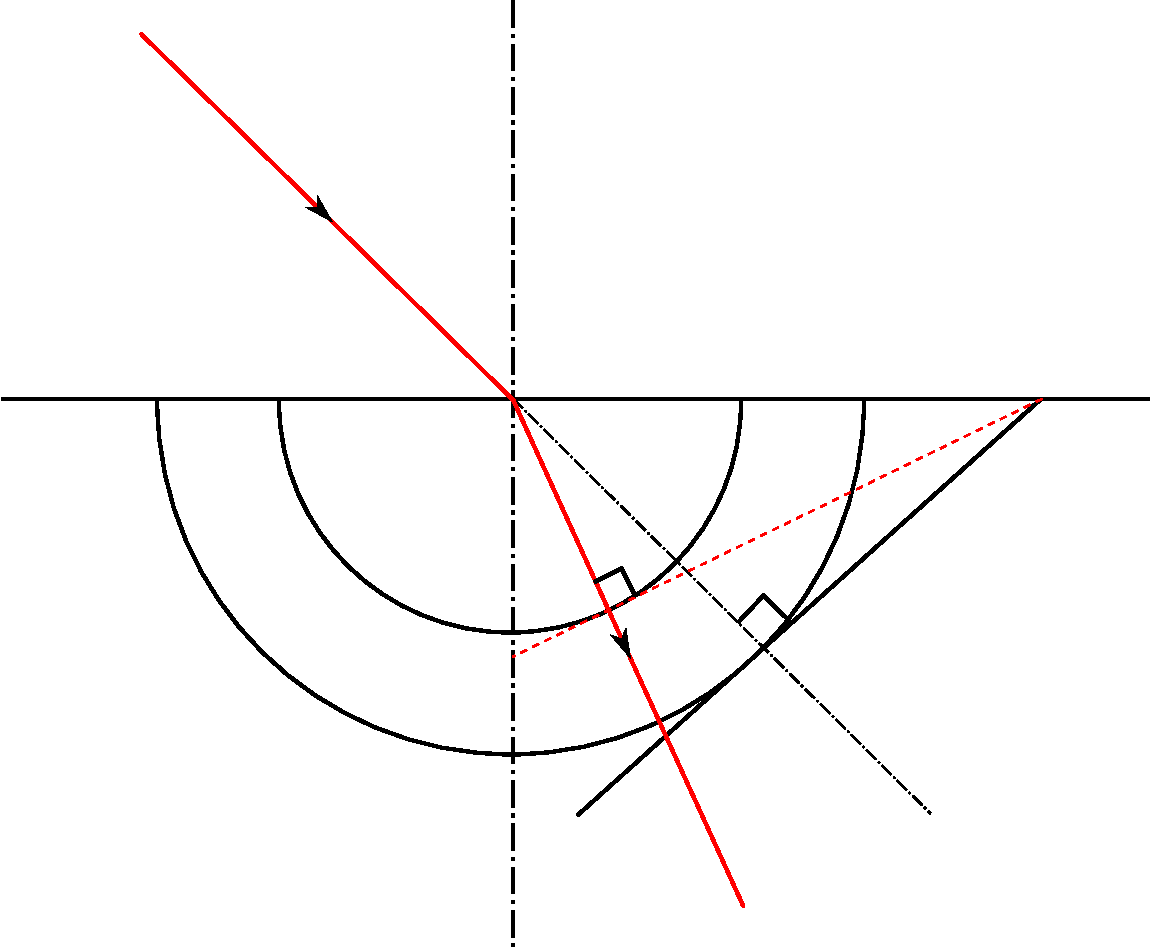
\includegraphics[height=10cm]{huygens.pdf}}
\put(0,6){\)n_1\)}
\put(0,5.5){\)n_2\)}
\end{picture}
\caption{Construction de Huygens}
\end{figure}
\end{verbatim}

\subsubsection{Astuce}
Pour trouver rapidement les coordonnées des points où l'on veut rajouter du texte, on peut ajouter temporairement un quadrillage en espaçant des traits plein tout les centimètres et des pointillés tout les demi-centimètres. Ceci marche dans mon cas puique l'unité de longueur est le centimètre et que je met mes figures dans un cadre de $10$ par $10$. À vous d'adapter suivant votre cas :

\begin{verbatim}
\multiput(0,0)(1,0){11}{\line(0,1){10}}
\multiput(0.5,0)(1,0){10}{\multiput(0,0)(0,0.2){50}{\line(0,1){0.1}}}
\multiput(0,0)(0,1){20}{\line(1,0){10}}
\multiput(0,0.5)(0,1){10}{\multiput(0,0)(0.2,0){50}{\line(1,0){0.1}}}
\end{verbatim}

\subsection{Superposer deux figures}\label{sec:superposition-figure}
\begin{verbatim}
 \noindent\hfill\makebox[0pt]{\includegraphics{A}}%
\makebox[0pt]{\includegraphics{B}}%
\hfill\null
\end{verbatim}
Ça ne fonctionne pas si la deuxième image n'a pas une largeur nulle elle aussi (ce qui ne me semblait pas logique au départ). Les \verb|\hfill| sont là pour forcer les images à être dans la page. Car comme on les définit avec une largeur nulle, la moitié de l'image sort du cadre à gauche si on ne fait rien.

Une autre solution est de faire : 
\begin{verbatim}
\makebox[0pt][l]{\includegraphics[width=0.9\textwidth]{Base.pdf}}%
\makebox[0pt][l]{\includegraphics[width=0.9\textwidth]{superp.pdf}}
\end{verbatim}
Sans le pourcentage entre les deux figures, les espaces ne sont pas rendus correctement, et il y a un petit décalage vers la droite de la 2\ieme image par rapport à la première.

\subsection{Gérer les tailles de figures}
J'avais pris l'habitude d'ajouter les figures, et de spécifier, quand j'en avais besoin, la largeur ou la hauteur en centimètre. Il est pourtant possible de gérer la largeur beaucoup plus proprement, notament si on oscille entre le mode page, et le mode deux colonnes.

Pour celà, on utilise \verb|[width=0.8\linewidth]| qui spécifie à \LaTeX{} que la figure doit être redimensionnée pour que la largeur de la figure fasse \(0.8\) fois la largeur de la ligne, en clair, la largeur de la page. Et si entre temps on passe en mode colonne, la figure est redimensionnée à la largeur de la colonne.

De plus, si on utilise le mode deux colonnes et que l'on utilise \verb|\begin{figure*}| la figure s'affiche sans tenir compte des colonnes (pas testé personnellement, mais il parait)

\subsection{Mettre plusieurs figures à coté}
Il faut pour celà utiliser le paquet \gras[package!subfig]{subfig}

\begin{scriptsize}\begin{verbatim}
\begin{figure}[htb]
\centering
\subfloat[1\ier{} figure]{\label{fig:figure1}
\includegraphics[width=0.2\textwidth]{figure/logo-ubuntu.pdf}}\hfill
\subfloat[2\ieme{} figure]{\label{fig:figure2}
\includegraphics[width=0.2\textwidth]{figure/logo-debian.pdf}}
\caption{Voici plusieurs figures dans un même environnement}
\end{figure}
\end{verbatim}\end{scriptsize}

\begin{remarque}
La commande \verb|\hfill| permet d'optimiser l'espacement entre les figures. C'est surtout pratique quand il y a plus de deux figures sur la même ligne. Ça permet, pour deux figures, d'aligner la première à gauche, et la deuxième à droite.
\end{remarque}


\begin{figure}[htb]
\centering
\subfloat[1\ier{} figure]{\label{fig:figure1}
\includegraphics[width=0.2\textwidth]{figure/logo-ubuntu.pdf}}\hfill
\subfloat[2\ieme{} figure]{\label{fig:figure2}
\includegraphics[width=0.2\textwidth]{figure/logo-debian.pdf}}
\caption{Voici plusieurs figures dans un même environnement}
\end{figure}


On peut appeler les figures avec des références séparées, ou rajouter un \gras[macro!label]{label} à droite du \gras[macro!caption]{caption} pour faire référence à tout le groupe.

\subsection{Fondre une figure dans un paragraphe}
Il faut pour celà utiliser le paquet \gras[package!floatflt]{floatflt} (il en existe cependant d'autres).

\begin{example}
\begin{floatingfigure}[l]
{0.3\linewidth}
\includegraphics[width=0.3\linewidth]%
{figure/logo-ubuntu.pdf}
\caption{Logo d'Ubuntu}
\end{floatingfigure}
du texte du texte du texte du texte
du texte du texte du texte du texte
du texte du texte du texte du texte
du texte du texte du texte du texte
du texte du texte du texte du texte
du texte du texte du texte du texte
du texte du texte du texte du texte
du texte du texte du texte du texte
du texte du texte du texte du texte
du texte du texte du texte du texte
du texte du texte du texte du texte
du texte du texte du texte du texte
\end{example}

\section{Mathématiques}
\subsection{Commandes utiles}
\begin{example}
\begin{align}
 f(x) & = x^2 + 8x + 16 \\
 & = (x+4)^2
\end{align}

\begin{align}
a&=1 & b&=2\\
c&=3 & d&=4
\end{align}

\end{example}

Permet d'aligner en colonne. Mettre une "*" permet d'enlever la numérotation des équations. En mettant un \verb|\notag|, on supprime la numérotation d'une seule ligne. En répétant les signes  \og\&\fg, on peut alors mettre en page plusieurs équations sur la même ligne. Les \og\&\fg impairs séparent les deux membres d'une équation tandis que les \og\&\fg pairs séparent les équations

\begin{example}
$\stackrel{\mathrm{d\acute ef}}{=}$

$\sum_{\substack{i=1\\ i\neq j}}$
\end{example}

permet de mettre deux chaines de caractères l'une au dessus de l'autre. (du genre dans ce cas, un \textbf{déf} au dessus d'un signe égal)

\subsection{Définitions à choix multiples (accolade)}

\begin{example}
\begin{align}
  f(x)&=
  \begin{cases}
    f(x_0)  & \text{si }  x<x_0\\
    f(x_1) & \text{si }  x_0<x<x_1\\
    f(x_2) & \text{si }  x>x_1
  \end{cases}
\end{align}
\end{example}
permet de faire une accolade avec des cas, le \og\&\fg aligne une deuxième partie.

\subsection{Exposant, indice}\index{exposant}\index{indice}

Pour mettre du texte en exposant, on place le texte dans un bloc et on le fait précéder d'un chapeau \verb|^|.

Pour mettre du texte en indice, on place le texte dans un bloc et on le fait précéder d'un tiret de soulignement  \verb|_| .

par exemple :

\begin{example}
\begin{align*}
u_n = 2^n \\
u_n+1 = 2^n+1 \\
u_{n+1} = 2^{n+1}
\end{align*}
\end{example}

On peut placer un objet au-dessus ou en dessous d'un autre.

\begin{example}
\begin{align*}
\overset{a}{X}\\
\underset{b}{X}\\
\overset{a}{\underset{b}{X}}
\end{align*}
\end{example}

\subsection{Faire des flèches adaptées à la longueur d'un texte}
La commande ci-dessous permet de générer des flèches dont la
longueur dépend de la longueur du texte qui est placé au dessus
ou en dessous (ou de la chaîne la plus longue lorsqu'il y a à la
fois un texte au dessus et un autre en dessous).

\begin{example}
\(\xrightarrow[\text{en dessous}]%
{\text{au dessus}}\)
\end{example}

\subsection{Les matrices}\index{matrice}
Ce sont des environnements à utiliser en mode mathématique.

\begin{tabular}{>{\bfseries}r<{}@{ : }p{11cm}}
matrix &  est une matrice sans aucun encadrement\\
pmatrix &  est une matrice entourée de parenthèses\\
bmatrix &  est une matrice entourée de crochets\\
vmatrix &  est une matrice entourée de barres verticales\\
Vmatrix &  est une matrice entourée de doubles barres verticales\\
\end{tabular}

% \begin{description}
% \item[matrix] est une matrice sans aucun encadrement
% \item[pmatrix] est une matrice entourée de parenthèses
% \item[bmatrix] est une matrice entourée de crochets
% \item[vmatrix] est une matrice entourée de barres verticales
% \item[Vmatrix] est une matrice entourée de doubles barres verticales
% \end{description}

\begin{example}
\[\begin{vmatrix}
  a & b\\
c & d
  \end{vmatrix}\]
\end{example}

\subsection{Mettre en page des équations}
\subsubsection{Pour commencer}
Quelques commandes \LaTeX{} utiles sont disponibles sous forme de paquets nommés \gras[package!amsmath]{amsmath}. Ils peuvent être chargés sur la plupart des installations de \LaTeX{} en plaçant dans le préambule de votre document cette commande.

Une commande très utile rend possible, au moyen de ces paquets, l'alignement des objets, par exemple le signe d'égalité \og=\fg sur des lignes d'équations successives. Voici un exemple :

\begin{example}
\begin{align}
x &= a + (b + a) \\
&= 2a + b.
\end{align}
\end{example}

Le symbole esperluette \og\&\fg est utilisé pour préciser les points dans chaque ligne qui seront supposés être alignés verticalement, mais n'apparaissent pas dans le résultat final.

Les équations sont numérotées par défaut. Les numéros d'équation peut être supprimés en remplaçant le mot \textbf{align} par le mot \textbf{align*} au début et à la fin des équations à aligner :

\begin{example}
\begin{align*}
x &= a + (b + a) \\
&= 2a + b.
\end{align*}
\end{example}

Une autre solution est de les supprimer sur une ligne particulière en ajoutant l'expression \verb|\notag|, comme nous le montrons ici :

\begin{example}
\begin{align}
x &= a + (b + a) \notag \\
&= 2a + b.
\end{align}
\end{example}

Des annotations dans chaque ligne peuvent être ajoutées en les séparant des équations, en utilisant deux esperluettes \og\&\&\fg :

\begin{example}
\begin{align}
x &= a + (b + a) && \text{Axiome C} \\
&= 2a + b && \text{Axiomes A \& F}.
\end{align}
\end{example}

\begin{remarque}
L'environnement \gras[macro!align]{align} est fait pour mettre en page plusieurs équations sur la même ligne. Ainsi, les colonnes sont alternativement alignés à droite et à gauche pour pouvoir aligner chaque colonne d'équations sur les signes de relation. De plus, chaque colonne alignée à droite a un espace important avec la colonne immédiatement précédente, ceci pour séparer les différentes colonnes d'équations. D'où la présence des deux esperluettes dans l'exemple précédent. En effet, la première donne un espace important, mais un alignement à droite ; or on veut que les commentaires commencent au même endroit, d'où la présence de la 2\ieme esperluette.
\end{remarque}


\subsubsection{Sous-équations}\label{sec:subequation}
Il s'avère souvent pratique, lorsqu'on a un ensemble d'équations se rapportant plus ou moins à la même chose, de les numéroter de la même manière de la façon suivante :

\begin{example}
\begin{subequations}
\begin{align}
x &= a + (b + a) \\
y&= 2c + d
\end{align}
\end{subequations}
\end{example}

\subsubsection{Mettre en page de longues équations}
On peut utiliser \gras[environnement!split]{split} :

\begin{example}
\begin{equation}\label{e:barwq}
\begin{split}
H_c&=\frac{1}{2n} \sum^n_{l=0}%
(-1)^{l}(n-{l})^{p-2}
\sum_{l _1+\dots+ l _p=l}%
\prod^p_{i=1} \binom{n_i}{l _i}\\
&\quad\cdot[(n-l )%
-(n_i-l _i)]^{n_i-l _i}\cdot
\Bigl[(n-l )^2-\sum^p_{j=1}%
(n_i-l _i)^2\Bigr].
\end{split}
\end{equation}
\end{example}

Ou encore dans cet exemple suivant qui numérote des sous équations, et en plus, met en page une longue équation (la deuxième) :

% \begin{example}
% \begin{subequations}
% \begin{align}
% E_n&= E_n^0+W\ket{\varphi_n}\\
% \begin{split}
% \ket{\psi_n}&= [1-\inv{2}]\ket{n}\\
% &+\sum_{p\neq n}\ket{n}
% \end{split}
% \end{align}
% \end{subequations}
% \end{example}

\begin{footnotesize}\begin{verbatim}
\begin{subequations}
\begin{align}
E_n&= E_n^0+\bra{\varphi_n}W\ket{\varphi_n}+\sum_{p\neq n}\frac{\abs{\bra{\varphi_p}W\ket{\varphi_n}}^2}%
{E_n^0-E_p^0}\\
\begin{split}
\ket{\psi_n}&= \left[1-\inv{2}\sum_{p\neq n}\frac{\abs{\bra{\varphi_p}W\ket{\varphi_n}}^2}{E_n^0-E_p^0}%
\right]\ket{\varphi_n}\\
&+\sum_{p\neq n}\left\{\frac{\bra{\varphi_p}W\ket{\varphi_n}}{E_n^0-E_p^0}+\sum_{p'\neq n}%
\frac{\bra{\varphi_{p'}}W\ket{\varphi_n}\bra{\varphi_p}W\ket{\varphi_{p'}}}{(E_n^0-E_p^0)(E_n^0-E_{p'}^0)}%
-\frac{\bra{\varphi_n}W\ket{\varphi_n}\bra{\varphi_p}W\ket{\varphi_n}}{E_n^0-E_p^0}\right\}
\end{split}
\end{align}
\end{subequations}
\end{verbatim}\end{footnotesize}

\begin{subequations}
\begin{align}
E_n&= E_n^0+\bra{\varphi_n}W\ket{\varphi_n}+\sum_{p\neq n}\frac{\abs{\bra{\varphi_p}W\ket{\varphi_n}}^2}{E_n^0-E_p^0}\\
\begin{split}
\ket{\psi_n}&= \left[1-\inv{2}\sum_{p\neq n}\frac{\abs{\bra{\varphi_p}W\ket{\varphi_n}}^2}{E_n^0-E_p^0}\right]\ket{\varphi_n}\\
&+\sum_{p\neq n}\left\{\frac{\bra{\varphi_p}W\ket{\varphi_n}}{E_n^0-E_p^0}+\sum_{p'\neq n}\frac{\bra{\varphi_{p'}}W\ket{\varphi_n}\bra{\varphi_p}W\ket{\varphi_{p'}}}{(E_n^0-E_p^0)(E_n^0-E_{p'}^0)}-\frac{\bra{\varphi_n}W\ket{\varphi_n}\bra{\varphi_p}W\ket{\varphi_n}}{E_n^0-E_p^0}\right\}
\end{split}
\end{align}
\end{subequations}

\bigskip

Et un dernier exemple pour montrer comment faire usage de \verb|\left(| et \verb|\right)| dans un environnement \gras[environnement!split]{split}

\begin{verbatim}
\begin{align*}
\begin{split}
F&=\left|\cos\left(2\sqrt{\Delta^2+\abs{W_{12}}^2} \sfrac{t}{\hbar}\right)
-i\cancel{\sin\left(2\sqrt{\Delta^2+\abs{W_{12}}^2} \sfrac{t}{\hbar}\right)}\right.\\
&\left.+\cos\left(2\sqrt{\Delta^2+\abs{W_{12}}^2} \sfrac{t}{\hbar}\right)
+i\cancel{\sin\left(2\sqrt{\Delta^2+\abs{W_{12}}^2} \sfrac{t}{\hbar}\right)}-2\right|
\end{split}
\end{align*}
\end{verbatim}



\begin{align*}
\begin{split}
F&=\left|\cos\left(2\sqrt{\Delta^2+\abs{W_{12}}^2} \sfrac{t}{\hbar}\right)-i\cancel{\sin\left(2\sqrt{\Delta^2+\abs{W_{12}}^2} \sfrac{t}{\hbar}\right)}\right.\\
&\left.+\cos\left(2\sqrt{\Delta^2+\abs{W_{12}}^2} \sfrac{t}{\hbar}\right)+i\cancel{\sin\left(2\sqrt{\Delta^2+\abs{W_{12}}^2} \sfrac{t}{\hbar}\right)}-2\right|
\end{split}
\end{align*}

Un exemple similaire montrant comment uniformiser la taille des parenthèses à l'aide de la commande \gras[macro!vphantom]{vphantom} qui permet d'introduire une hauteur fantôme d'une suite de caractères donnés, sans pour autant les imprimer à l'écran :

\begin{verbatim}
\begin{align}
\begin{split}
E&=\left(2+\vphantom{\frac{2}{\frac{2}{3}}}\right.\\
&\left.\frac{2}{\frac{2}{3}}\right)
\end{split}
\end{align}
\end{verbatim}

\begin{align}
\begin{split}
E&=\left(2+\vphantom{\frac{2}{\frac{2}{3}}}\right.\\
&\left.\frac{2}{\frac{2}{3}}\right)
\end{split}
\end{align}




\subsubsection{Aligner des équations terme à terme}
La solution que j'ai trouvée est d'utiliser l'environnement \gras[macro!alignat]{alignat} pour lequel le nombre entre accolade correspond au nombre de colonnes :

\begin{footnotesize}\begin{verbatim}
\begin{alignat}{4}
\dif U&= \left ( \pd{U}{S}\right )_{V,N}&&\dif S +\left ( \pd{U}{V}\right )_{S,N}%
&&\dif V +\left ( \pd{U}{N}\right )_{S,V}&&\dif N\\
&= T&&\dif S-p&&\dif V+\mu&&\dif N
\end{alignat}
\end{verbatim}\end{footnotesize}

\begin{alignat}{5}
\dif U&= \left ( \pd{U}{S}\right )_{V,N}&&\dif S +\left ( \pd{U}{V}\right )_{S,N}&&\dif V +\left ( \pd{U}{N}\right )_{S,V}&&\dif N\\
&= T&&\dif S-p&&\dif V+\mu&&\dif N
\end{alignat}

\begin{remarque}
Vous aurez sans doute remarqué que le nombre passé en argument à \gras[macro!alignat]{alignat} ne vaut pas du tout le nombre d'esperluette (\&). En effet, cet environnement est au départ prévu pour aligner $n$ équations (tout comme \gras[macro!align]{align}, sauf qu'il ne met pas des espaces gigantesques) sur une même ligne. On sépare les équations par un \og\&\fg, et à chaque équation est associé un \og\&\fg supplémentaire qui doit être placé avant le symbole de relation. Chaque \og\&\fg impaire aura donc la partie de gauche justifiée à droite, et la partie de droite justifiée à gauche (ainsi, l'équation est bien accolée au symbole de relation).

Dans notre cas, pour aligner des parties d'une seule équation, on utilise la double esperluette, afin que l'on ai un alignement correct des termes.
\end{remarque}

\subsubsection{Insérer du texte entre deux équations d'un même environnement}
La commande \gras[macro!intertext]{intertext} est très utile quand on veut placer du texte entre deux lignes d'équations sans sortir de l'environnement mathématique comme le montre l'exemple suivant :


\begin{equation}
\begin{split}
A_{1} & = \left| \int _{0}^{1}(f(x)-g(x))\dif x\right| +\left| \int _{1}^{2}(g(x)-h(x))
\dif x\right| \\
 & = \left| \int _{0}^{1}(x^{2}-3x)\dif x\right| +\left| \int _{1}^{2}(x^{2}-5x+6)
\dif x\right| \\
\intertext{Now the limits of the integrals are used}
& = \left| \frac{x^{3}}{3}-\frac{3}{2}x^{2}\right| _{0}^{1}+\left| \frac{x^{3}}{3}-
\frac{5}{2}x^{2}+6x\right| _{1}^{2}\\
& = \left| \frac{1}{3}-\frac{3}{2}\right| +\left| \frac{8}{3}-\frac{20}{2}+12-
\left( \frac{1}{3}-\frac{5}{2}+6\right) \right| \\
& = \left| -\frac{7}{6}\right| +\left| \frac{14}{3}-\frac{23}{6}\right| =\frac{7}{6}+
\frac{5}{6}=2\, \textrm{FE}
\end{split}
\end{equation}

Le code est le suivant :

\begin{footnotesize}\begin{verbatim}
\begin{equation}
\begin{split}
A_{1} & = \left| \int _{0}^{1}(f(x)-g(x))\dif x\right| +\left| \int _{1}^{2}(g(x)-h(x))
\dif x\right| \\
 & = \left| \int _{0}^{1}(x^{2}-3x)\dif x\right| +\left| \int _{1}^{2}(x^{2}-5x+6)
\dif x\right| \\
\intertext{Now the limits of the integrals are used}
& = \left| \frac{x^{3}}{3}-\frac{3}{2}x^{2}\right| _{0}^{1}+\left| \frac{x^{3}}{3}-
\frac{5}{2}x^{2}+6x\right| _{1}^{2}\\
& = \left| \frac{1}{3}-\frac{3}{2}\right| +\left| \frac{8}{3}-\frac{20}{2}+12-
\left( \frac{1}{3}-\frac{5}{2}+6\right) \right| \\
& = \left| -\frac{7}{6}\right| +\left| \frac{14}{3}-\frac{23}{6}\right| =\frac{7}{6}+
\frac{5}{6}=2\, \textrm{FE}
\end{split}
\end{equation}
\end{verbatim}\end{footnotesize}

Écrire un long texte est possible en utilisant la commande \gras[macro!parbox]{parbox}

\begin{verbatim}
\begin{align}
a+b+c+d+ef & = g+h+i+j+k %
&\textrm{\parbox[t]{.25\linewidth}{%
this is a very long description of a formula}%
}
\end{align}
\end{verbatim}

\subsubsection{Insérer une \texttt{footnote} dans une équation}\index{macro!footnote}\index{macro!footnotetext}

Dans l'environnement \verb|\[ \]| ou \textbf{equation}, \LaTeX{} n'accepte pas la syntaxe \verb|\footnote{}|. Il faut donc marquer avec \gras[macro!footnotemark]{footnotemark} comme le montre l'exemple suivant :
\begin{example}
\begin{align}
\cte&=-i\omega \frac{x}{v}\\
\intertext{On sait de plus que pour une %
onde on a $v=\frac{\omega}{k}$\footnotemark}
\cte&=-i\omega \frac{x}{\frac{\omega}{k}}
\end{align}
\footnotetext{o\'{u} $k$ est la norme du%
vecteur d'onde}
\end{example}

\subsubsection{Simplifier des termes d'une équation}
Le paquet \gras[package!cancel]{cancel} permet d'utiliser trois commandes différentes pour simplifier les termes d'une équation ; très pratique pour représenter visuellement des simplifications dans une équation.

Le paquet \gras[package!cancel]{cancel} est présenté dans le paragraphe \ref{sec:cancel}.

\subsubsection{Ce qu'il ne faut pas utiliser et pourquoi}
Il existe un environnement appelé \gras[macro!eqnarray]{eqnarray} qui permet de mettre en page des équations, de les numéroter, et d'aligner des signes d'égalité. Cependant, celui-ci souffre de plusieurs défauts :
\begin{enumerate}
\item Il rajoute beaucoup d'espacement autour du symbole de relation, de façon injustifiée et incohérente avec les autres environnements.
\item Quand l'équation occupe toute la largeur de la page, \gras[macro!eqnarray]{eqnarray} ne s'en rend pas compte et place le numéro d'équation en surimpression sur le texte. Les autres environnements standard, comme \gras[macro!equation]{equation}, ne présentent pas ce problème et placent le tag en-dessous.
\item Par ailleurs, eqnarray ne fonctionne pas correctement avec les commandes du package \gras[package!amsmath]{amsmath}, incontournable pour composer les mathématiques. Par exemple, les commandes \verb|\tag| et \verb|\intertext| fonctionnent avec tous les environnements sauf \gras[macro!eqnarray]{eqnarray}.
\end{enumerate}

L'usage de \verb|$$\dots $$| pour passer en mode mathématique hors-texte n'a jamais été supporté par \LaTeX{} : c'est un héritage de \TeX. Les héritages de \TeX{} ne sont pas tous mauvais, mais celui-ci est à éviter pour (au moins) les raisons suivantes :
\begin{enumerate}
\item Il ne respecte pas les mécanismes de \LaTeX, comme par exemple l'option fleqn de la classe standard article : cette dernière doit avoir pour effet d'aligner à gauche (au lieu de centrer) les équations hors-texte, mais les équations délimitées par \verb|$$| restent obstinément centrées.
\item L'espacement vertical autour de l'équation est inconsistant. La plupart du temps, il sera correct, mais des comportements étranges peuvent survenir quand l'équation est précédée ou suivie de changements de paragraphes ou autres objets \og complexes \fg.
\item Enfin, tous les packages bien faits pour \LaTeX{} supposent que vous utilisez les constructions standard de \LaTeX, et risquent donc de ne pas fonctionner avec \verb|$$|. C'est le cas d'\gras[package!amsmath]{amsmath}, et par exemple, de sa commande \verb|\tag|.
\end{enumerate}

Les environnement standard prévus par \LaTeX{} pour les mathématiques hors-texte sont \gras[macro!displaymath]{displaymath}, \gras[macro!equation*]{equation*} et \verb|\[\dots \]| : le dernier n'est guère plus long à taper que \verb|$$| et rend par ailleurs le source plus lisible en différenciant l'ouverture de la fermeture du mode math.

\begin{remarque}
Il existe l'environnement \gras[macro!equation]{equation}, mais celui-ci ne permet de faire qu'une seule équation ce qui limite beaucoup les possibilités.

Par ailleurs, il est souvent pratique de faire des sous numérotations, comme le fait \gras[macro!subeqnarray]{subeqnarray}, mais nous l'avons vu plus haut, les environnements \gras[macro!eqnarray]{eqnarray} ne doivent pas être utilisés, il faut donc utiliser autre chose à la place. Pour celà, se référer à la section \refsec{sec:subequation}.
\end{remarque}


% \subsection{Numéroter des équations}
% L'exemple ci-dessous permet de numéroter des équations. Je ne sais pas s'il nécessite l'utilisation d'un package particulier, si c'est le cas, c'est peut-être \gras[package!amsmath]{amsmath}. Ça permet d'en numéroter plusieurs à la fois.
%
% \begin{example}
% \begin{eqnarray}
% \delta(\alpha x)=\inv{\abs{a}}\delta(x)\\
% g(x)\delta(x-a)=g(a)\delta(x-a)\\
% \delta\left [g(x)\right ]=
% \sum_i\inv{\abs{g'(a_i)}}\delta(x-a_i)
% \end{eqnarray}
% \end{example}
%
% On peut aussi numéroter plusieurs équations d'une autre manière, en les regroupants si elles représentent par exemple plusieurs équations du même type. Il peut être intéressant de les grouper. Il faut utiliser le package \gras[package!subeqnarray]{subeqnarray}.
%
% \begin{example}
% \begin{subeqnarray}
% \delta(\alpha x)=\inv{\abs{a}}\delta(x)\\
% g(x)\delta(x-a)=g(a)\delta(x-a)\\
% \delta\left [g(x)\right ]=
% \sum_i\inv{\abs{g'(a_i)}}\delta(x-a_i)
% \end{subeqnarray}
% \end{example}
%
% Pour ne pas numéroter une ligne en particulier, on peut utiliser la commande \verb|\nonumber| avant le \verb|\\|. Pour que l'environnement ne numérote aucune équations, il faut utiliser une version étoilée de l'environnement, comme pratiquement tout les environnements d'ailleurs
%
% \begin{example}
% \begin{eqnarray*}
% \delta(\alpha x)=\inv{\abs{a}}\delta(x)\\
% g(x)\delta(x-a)=g(a)\delta(x-a)\\
% \end{eqnarray*}
% \end{example}

\subsection{Mise en forme des vecteurs}
Il existe principalement deux manières de noter des vecteurs. Soit un mettant une flèche sur le symbole (manière plutôt française), soit en mettant le caractère en gras (plutôt anglosaxonne). En \LaTeX, après plusieurs péripéties, j'ai trouvé une manière relativement proprement de mettre en gras les vecteurs :
\begin{example}
\[\boldsymbol{\nabla}f=\boldsymbol{0}\]
\end{example}

Personnellement, j'ai été habitué à noter les vecteurs avec des flèches. En écrivant à la main, on fait ça, alors pourquoi ne pas continuer par ordinateur? Pour faire une flèche, j'utilise :
\begin{example}
\[\overrightarrow{\nabla}f=\overrightarrow{0}\]
\end{example}

Chaque méthode a ses avantages et ses inconvénients. Pour ma part, j'ai adopté la technique suivante : j'ai définit une commance \verb|\vect{}|. Et suivant les besoins, je pourrais définir deux versions de ma commande :
\begin{verbatim}
\newcommand{\vect}[1]{\overrightarrow{#1}}
%ou
%\newcommand{\vect}[1]{\boldsymbol{#1}}
\end{verbatim}

Il fut un temps où la définition de ma commande était la suivante :
\begin{verbatim}
\newcommand{\vect}[1]{\overrightarrow{#1\mathstrut}}
\end{verbatim}
\verb|\mathstrut| permet d'aligner les différentes flèches des vecteurs entre elles. C'est vrai que c'est plus joli, mais, d'une manière générale, ça relève énormément les flèches par rapport aux symboles juste en dessous d'eux, et finalement, j'en suis venu à penser que c'est pas si esthétique que ça.


\subsection{Symboles Utiles}
% \displaystyle : permet d'afficher des formules de math en mode en texte comme si elles étaient en hors texte.

\begin{example}
\begin{align*}
\int_0^{+\infty}x^2\dif x\\
\oint_\mathscr{C}\dif \varphi\\
\iint_S\dif r \dif \theta\\
x\in\mathbb{R}\\
\abs{x}\\
\norm{x}\\
\mathscr{L}\\
\binom{n}{k}\\
\approx\\
\boxed{x^2=3}
\end{align*}
\end{example}

\begin{example}
\AA
\end{example}

% \DeclareMathOperator{\rank}{rank} : permet de déclarer un nouvel opérateur mathématique comme cos ou sin.

% \mathstrut : permet d'aligner les différentes occurences d'une chose, style la flèche d'un vecteur s'il est placé juste avant l'accolade de fin de chaque groupe qui les constituent

\section{Physique}
Dans cette section je détaillerais les commandes à utiliser pour certaines fonctions ou notations.

\subsection{Flèche du comportement asymptotique}
Quand on veut mettre en page un comportement asymptotique d'une fonction, il est parfois difficile de mettre en dessous de la flèche vers quoi tend la variable. Voici la solution que j'utilise :
\begin{example}
\begin{align}
f(x)\xrightarrow[x\to 0]{}x
\end{align}
\end{example}


\subsection{Slash de Feynman}\index{slash de feynman}
Une des solutions est d'utiliser la commande \verb|\not| devant, mais celle-ci n'est pas satisfaisante. La commande à utiliser est \verb|\slashed{}|, de la façon suivante :
\begin{example}
\begin{align*}
(i\slashed{\partial} -m)\psi(\underline{x})&=0
\end{align*}
\end{example}

Pour pouvoir utiliser cette macro, il faut ajouter le paquet \gras[package!slashed]{slashed}.



\section{Packages}
\subsection{acronym}
Le paquet \gras[package!acronym]{acronym} permet de définir, comme son nom l'indique, des acronymes tels \bsc{sncf}. Il permet de définir la version courte et longue d'un acronyme, et on appelle ainsi l'un ou autre, ou les deux pour sa première apparition.

En fin de document, ou du moins, dans le document, il faut introduire l'environnement \gras[macro!acronym]{acronym}. Celui-ci contiendra toutes les définitions d'acronymes. À l'intérieur de l'environnement, on peut utiliser la commande \verb|\acro| pour définir un acronyme qui sera affiché dans la liste d'acronyme, ou \verb|\acrodef| pour définir l'acronyme sans que celui-ci ne soit affiché dans la liste.

Voici un exemple :

\begin{small}\begin{verbatim}
\begin{acronym}[TDMA]
\acro{CDMA}{Code Division Multiple Access}
\acro{GSM}{Global System for Mobile communication}
\acro{NA}[\ensuremath{N_{\mathrm A}}]{Number of Avogadro\acroextra{ (see \S ref)}}
\acro{NAD+}[NAD\textsuperscript{+}]{Nicotinamide Adenine Dinucleotide}
\acro{NUA}{Not Used Acronym}
\acro{TDMA}{Time Division Multiple Access}
\acro{UA}{Used Acronym}
\acro{lox}[\ensuremath{LOX}]{Liquid Oxygen}%
\acro{lh2}[\ensuremath{LH_2}]{Liquid Hydrogen}%
\end{acronym}
\end{verbatim}\end{small}

\begin{remarque}
Juste après la définition de l'environnement, on peut remarquer \textbf{[TDMA]}, ceci permet de définir une largueur pour la \og colonne \fg de la définition courte des acronymes. En effet, on voit que \bsc{TDMA} est le sigle le plus long de l'environnement, on le définit donc comme largueur limite pour aligner la colonne suivante à partir de cette largueur là.

Il y a de plus un paramètre optionnel qui permet de définir la définition courte de l'acronyme, si celle-ci diffère par rapport à l'identifiant de l'acronyme lorsqu'on l'appellera dans le code source du document. Concrêtement, ça sert quand le sigle est compliqué, et/ou défini en mode mathématique avec des exposants ou indices.
\end{remarque}

Pour être plus clair, j'appelle \textbf{full} le développement de l'acronyme, et \textbf{short} son sigle correspondant. Pour appeler un acronyme dans le document, on a 4 commandes :

\begin{tabular}{r@{ : }p{11cm}}
\verb|\ac{acronym}|  &	Pour identifier l'acronyme à sa première utilisation. Cette commande renvoie le sigle suivie de sa signification (\textbf{full} + \textbf{short}).\\
\verb|\acf{acronym}| &	Affiche le développement complet de l'acronyme. (\textbf{full} + \textbf{short})\\
\verb|\acs{acronym}| &	Affiche la version courte de l'acronyme, même si cette commande est utilisée avant son \verb|\ac| correspondant (\textbf{short})\\
\verb|\acl{acronym}| &	Développe l'acronyme sans afficher la version courte. (\textbf{full})
\end{tabular}


\subsection{babel}\label{babel}\index{package!babel}

Il est généralement utilisé par défaut pour permettre l'affichage correct des accents et cie dans la langue française et faciliter la rédaction du source en écrivant les accents directement dans le source. Il est appelé la plupart du temps ainsi :

\begin{verbatim}
\usepackage[frenchb]{babel}
\end{verbatim}

\subsubsection{Les acronymes, siglaisons et nom propres}

\gras[package!babel]{babel} propose la commande \verb|\bsc| pour placer un bout de texte en petites capitales. Cela peut être pratique pour les acronymes, siglaisons et les noms propres.

Exemple :
\begin{example}
La \bsc{sncf} embauche Jacques \bsc{Durand}.
\end{example}

\subsubsection{Les symboles divers}

\gras[package!babel]{babel} propose deux commandes pour afficher les degrés : \verb|\degre| et \verb|\degres|. La première sert pour les angles et la seconde pour les températures.

\begin{example}
pour afficher des angles : 30\degre\\
pour afficher des temperatures : 0\degres C
\end{example}

\subsubsection{1er, 2e, etc.}

\gras[package!babel]{babel} fournit les commandes suivantes pour les abbréviations de premier, deuxième, etc. : \verb|ier|, \verb|iers|, \verb|iere|, \verb|ieres|, \verb|ieme| et \verb|iemes|. Ces commandes sont pratiques car elles utilisent les bonnes règles d'affichage des ces abbréviations.

On peux aussi utiliser les commandes \verb|primo|, \verb|secundo|, \verb|tertio| et \verb|quarto|.

\begin{example}
1\ier, 1\iers, 1\iere, 1\ieres,\\
 2\ieme, 3\iemes\\
\primo, \secundo, \tertio, \quarto
\end{example}

\subsubsection{Écrire des grands nombres}
L'option \textbf{frenchb} de l'extension \gras[package!babel]{babel} fournit la commande \verb|\nombre| qui met en forme automatiquement les grands nombres : avant et après le séparateur décimal, les chiffres sont groupés par trois et ces groupes sont séparés par une espace. Par exemple :

\begin{example}
\nombre{123456,789123}
\end{example}

En particulier, hors du mode mathématique, la commande \verb|\nombre| permet de supprimer l'espace ajoutée après la virgule.

\begin{remarque}
Il faut maintenant inclure le package \gras[package!numprint]{numprint} et il est de plus conseillé d'utiliser \verb|\numprint{123456,789123}| à la place de \verb|\nombre{123456,789123}|
\end{remarque}

\subsection{cancel}\index{package!cancel}\label{sec:cancel}
Ce paquet permet de barrer de différentes manières des expressions, y compris en mode mathématique.

\begin{example}
\begin{align}
\dif G&=\cancel{T\dif S}%
-\bcancel{p\dif V}+\dots\\
&=\xcancel{p\dif V}\\
&=\cancelto{0}{p\dif V}
\end{align}
\end{example}

\begin{remarque}
Les commandes \gras[macro!cancel]{cancel}, \gras[macro!bcancel]{bcancel} et \gras[macro!xcancel]{xcancel} fonctionnent en mode math comme en mode texte. Par contre, la commande \gras[macro!cancelto]{cancelto} marche uniquement en mode mathématique.
\end{remarque}

Ce paquet permet par exemple de barrer des termes deux à deux pour qu'on voit plus facilement qui se simplifie avec qui (on peut donc simplifier au maximum trois ensembles, de manière différentes --- slash normal, anti-slash, et croix ) :
\begin{align}
\dif G&=\cancel{T\dif S}-\bcancel{p\dif V}+\mu\dif N-\cancel{T\dif S} -S\dif T+\bcancel{p\dif V}+V\dif p
\end{align}
\begin{verbatim}
\begin{align}
\dif G&=\cancel{T\dif S}-\bcancel{p\dif V}+\mu\dif N-\cancel{T\dif S}
-S\dif T+\bcancel{p\dif V}+V\dif p
\end{align}
\end{verbatim}


\begin{remarque}
Si on veut barrer une puissance ou tout autre objet qui nécessite des parenthèses si on veut inclure plusieurs caractères, il faut utiliser un groupe. C'est à dire qu'on doit faire ça
\begin{example}
\begin{align}
2^{\cancel{2}} x&=3\cdot\cancel{2}
\end{align}
\end{example}
\end{remarque}


\subsection{color}\index{package!color}
Ce package est l'équivalent des commandes de couleur pour \gras[package!pstricks]{pstricks}, ceci permettant d'utiliser les couleurs sans avoir à inclure le package \gras[package!pstricks]{pstricks} tout entier. Ci-dessous les commandes pour définir de nouvelles couleurs :
\begin{description}
 \item[gray] taux de gris. Il est défini par un nombre décimal compris entre 0 et 1 inclu, 0 correspondant au noir et 1 au blanc.
\item[rgb] correspond aux taux de rouge {1,0,0}, vert {0,1,0} et bleu {0,0,1}. Chaque taux correspondant à un nombre décimal compris entre 0 et 1 inclu.
\item[cmyk] cyan {1,0,0;0}, magenta {0,1,0;0}, jaune {0,0,1;0}, et noir {0,0,0;1}. Ce sera cette fois quatre nombres décimaux compris entre 0 et 1 inclu.
\end{description}

La définition d'une couleur se fait alors dans l'entête (ce n'est pas une obligation) par la commande \verb|\definecolor{nom}{modèle}{taux}|. Les différents taux sont séparés par une virgule (attention les nombres décimaux s'écrivent à l'anglaise, c'est à dire avec un \og.\fg). Pour donner un exemple plus concret, si je veux définir une couleur à 25\% de gris, j'utiliserai la ligne \verb|\definecolor{gris25}{gray}{0.75}|

Autre exemple : j'aimerais une sorte de violet, je me dis moitié-moitié de rouge et de bleu :

\begin{verbatim}
\definecolor{violet}{rgb}{0.5,0,0.5}
\end{verbatim}

Pour utiliser ces couleurs, on fait :

\begin{verbatim}
{\color{MyLightMagenta}This color is MyLightMagenta}
\end{verbatim}

\subsection{commath}\index{package!commath}

\begin{example}
\[\dif x\]
\end{example}

donne la différentielle de x, donc "dx"

\begin{example}
\[\od[2]{f}{x}\]
\end{example}

donne la dérivée d'ordre 2 de f par rapport à x, pour les dérivées premières, simplement oublier le [2] qui correspond à l'ordre de dérivation et qui par défaut vaut 1 (note:\verb|\tod| pour affichage en texte, \verb|\dod| pour affichage en hors texte)

\begin{example}
\[\pd[2]{f}{x}\]
\end{example}

donne la dérivée partielle d'ordre 2 de f par rapport à x, pour les dérivées partielles premières, simplement oublier le [2] qui correspond à l'ordre de dérivation et qui par défaut vaut 1 (note:\verb|\tpd| pour affichage en texte, \verb|\dpd| pour affichage en hors texte)

\begin{example}
\[\md{f}{5}{x}{2}{y}{3}\]
\end{example}

donne la dérivée partielles d'ordre 5 de f dérivée deux fois par rapport à x et 3 fois par rapport à y (note:\verb|\tmd| pour affichage en texte, \verb|\dmd| pour affichage en hors texte)

\begin{example}
\[\eval{f(\epsilon)}_{\epsilon=0}\]
\end{example}

affiche l'évaluation de \(f\) en \(\epsilon = 0\) (pour les décomposition en élément simple par exemple)

\begin{example}
\[\sVert[4]\]
\end{example}

affiche une barre verticale dont la hauteur est déterminée par la valeur (entière?) entre crochet.

\begin{remarque}
J'ai enlevé ce paquet de mes définitions car il entrait en conflit avec un paquet de toute ma liste de paquet, mais je ne sais pas lequel. En effet, à cause de ce conflit, je ne pouvais plus mettre de \og :\fg en mode mathématique, ce qui est relativement facheux.

Pour remédier à ça, j'ai redéfini les commandes du paquets dans mon paquet à moi, et depuis, plus de soucis.
\end{remarque}

\subsection{fancybox}\index{package!fancybox}
permet de d'encadrer du texte, si on veut encadrer des formules de maths, elles ne doivent pas être en hors texte, chose que l'on peut compenser par la macro \verb|\displaystyle| en début de formule mathématique.
\paragraph{doublebox}
\begin{example}
 \doublebox{texte}
\end{example}

\paragraph{fbox}

\begin{example}
 \fbox{texte}
\end{example}

\paragraph{shadowbox}
\begin{example}
 \shadowbox{texte}
\end{example}

\paragraph{ovalbox}
\begin{example}
 \ovalbox{texte}
\end{example}

\paragraph{Ovalbox}
\begin{example}
 \Ovalbox{texte}
\end{example}


\subsection{fancyhdr}\index{package!fancyhdr}

permet d'utiliser le pagestyle \og fancy\fg et de mieux gérer les header et footer

l pour left, r pour right, et c pour center qui permet de gérer trois parties de head et foot avec la syntaxe \verb|\lhead{} \chead{} \rhead{} lfoot{} cfoot{} rfoot{}|

\verb|\thepage| entre le numéro de la page en cours et \verb|\leftmark| affiche le titre de la section en cours (chapitre si en \gras[classe!report]{report}), et \verb|\rightmark| affiche le titre de la sous section en cours (section si en \gras[classe!report]{report}).

\verb|\fancyhead{}| permet d'effacer tout les champs du header

\verb|\fancyfoot{}| permet d'effacer tout les champs du footer

\verb|\fancyhf{}| permet d'effacer tout les champs des headers et footers bien sur dans l'optique de les redéfinir par la suite.

Pour afficher les titres en minuscules, il faut utiliser la syntaxe suivante :
\begin{verbatim}
\nouppercase{\leftmark}
\end{verbatim}

Voici un exemple d'entête utilisé avec l'option \gras{twoside} pour la classe (soit \gras[classe!report]{report}, soit \gras[classe!article]{article}) :
\begin{verbatim}
\fancyhead[LO,RE]{\thepage}
\fancyhead[RO]{\leftmark}
\fancyhead[LE]{\nouppercase{\rightmark}}
\end{verbatim}


\subsection{hyperref}\index{package!hyperref}
\begin{example}
 \url{http://google.fr/}
\end{example}

\subsection{ifsym}\index{package!ifsym}
Permet de tracer des diagrammes d'électroniques. Il faut ajouter certaines options parfois. dans mon cas, j'ai dû définir le package comme suit \verb|\usepackage[electronic]{ifsym}|

\begin{example}
\FallingEdge
\LongPulseLow
\PulseLow
\ShortPulseHigh
\LongPulseHigh
\PulseHigh
\RaisingEdge
\ShortPulseLow
\end{example}
Une commande pratique (la seule que je connais en fait) de ce package est \verb|\textifsym{}|, dont les commandes sont \verb|l m h d < > L M H D << >>|\par
\begin{example}
 \textifsym{mm<DDD>mm}\\
\textifsym{L|H|L|H|L}
\end{example}

\subsection{lettre}\index{package!lettre}\index{lettres}
Pour faire des lettres en français via \LaTeX, il est généralement conseillé d'utiliser le package \gras[package!lettre]{lettre}. Suite à quelques déconvenues dans son utilisation, voici quelques astuces et un exemple type de lettre que je fais :
\begin{verbatim}
\documentclass{lettre}
\usepackage[francais]{babel}
\usepackage[autolanguage]{numprint}
\usepackage{xspace}
\usepackage{amsmath}
\usepackage[utf8]{inputenc}
\usepackage[T1]{fontenc}

\institut{moi}
\begin{document}
% Eventuellement impression d'un logo

\begin{letter}{nom du destinataire\\
adresse du destinataire\\
\numprint{00000} \textsc{Ville}}

\conc{Objet de la lettre}

\opening{Madame, Monsieur,}

CONTENU DE LA LETTRE

\closing{Dans l'attente de votre réponse, je vous prie d'agréer, Madame, Monsieur,
l'expression de mes salutations distinguées.}

% \ps{P.S. : }
\end{letter}
\end{document}
\end{verbatim}

Le package \gras[package!numprint]{numprint} permet d'utiliser la commande \verb|\numprint| qui permet de mettre en forme des nombres (en espaçant correctement les milliers par exemple).

\begin{attention}
La commande \verb|\numprint{dsfkjh}| génèrera une erreur. Il faut absolument que l'argument de la commande \verb|\numprint| soit un nombre.
\end{attention}


\gras[package!xspace]{xspace} permet de bien espacer les guillemets et les choses de ce style. \gras[package!amsmath]{amsmath}, c'est juste parce que parfois j'utilise des maths dans mes lettres, mais pas utile pour vous si vous n'en faites pas. Les deux dernières lignes, inputenc et fontenc me permettent de dire que je rédige ma lettre en utf-8.

\verb|\institut{nom}| permet d'aller chercher un fichier \texttt{nom.ins} qui contiendra les noms, adresses, numéro de téléphone de la personne qui envoit la lettre, c'est à dire vous, en l'occurence. Pour exemple, voici mon fichier .ins :
\begin{verbatim}
\address{M. \textsc{Nom} Prénom\\
Lieu Dit : \og machin \fg\\
\numprint{72700} \textsc{Ville}}
\telephone{00 00 00 00 00}
\email{adresse@mail.com}
\signature{M. \textsc{Nom} Prénom}
\lieu{\textsc{Ville}}
% \notelephone
\nofax
\end{verbatim}


\subsection{listings}\index{package!listings}

Il s'utilise de la manière suivante :

\begin{verbatim}
\begin{lstlisting}[language={c++},title={nom du programme}]
#include <stdio.h>

int main(void)
{
int j=0, multiplication, entree=3;
  while (j <= 10)
    {
	multiplication = entree * j;
	printf ("%d x %d = %d\n", entree, j, multiplication);
	j++;
    }
  return 0;
}
\end{lstlisting}
\end{verbatim}


On peut modifier, via des options, l'affichage du code, les mots spéciaux et cie. Voici ce que je donne comme option à la suite de la déclaration du paquet :
\begin{verbatim}
\lstset{%
%Basic Appearance%
  basicstyle=\footnotesize\ttfamily,
  commentstyle=\itshape\color{gray},
  keywordstyle=\color{purple}\bfseries,
  stringstyle=\color{blue}\rmfamily,
%Basic Layout%
  tabsize=4,
  showtabs=false,
  showspaces=false,
  showstringspaces=false,
%Numbering%
  numbers=left,
  stepnumber=1,
  numberstyle=\scriptsize,
  numbersep=5pt,
%Margins%
  xleftmargin=0.02\textwidth,
  xrightmargin=0.02\textwidth,
  breaklines=true,
%Frame%
  frame=leftline,
  framerule=0.5pt,
  rulecolor=\color{purple},
  framexleftmargin=0em,
%Captions, Index, and so on passed as arguments%
  }
\end{verbatim}

\begin{remarque}
Il faut faire attention à ne pas trop modifier les choses. En particulier le caractère d'échappement pour pouvoir faire du \LaTeX. Ça peut donner des erreurs de compilation suivant les caractères qu'on met dans l'environnement \gras[environnement!lstlisting]{lstlisting}.
\end{remarque}


L'extension \gras[package!listings]{listings} permet de mettre du code source. On ne peut pas utiliser de caractères Unicode dans le code mise en forme par les commandes de cette extension.

Le code source est placé dans un environnement \gras[environnement!lstlisting]{lstlisting} ; la mise en forme stricte (y compris les espaces et les retours de ligne) est respectée, et les commandes \LaTeX{} ne sont pas interprétées.

\subsubsection{Options spécifiques pour un language}
On peut définir ou redéfinir un langage ainsi qu'un caractère d'échappement juste après l'appel de l'extension :
\begin{lstlisting}[language={TeX}]
\usepackage{listings}
\lstset{language=TeX,
   basicstyle=\ttfamily\small,
   columns=flexible,
   escapechar=+}
\end{lstlisting}

Dans l'exemple ci-dessus, on indique :

\begin{itemize}
\item que l'on écrit du \TeX{} ou du \LaTeX, ce qui permettra à l'extension de reconnaître les mots-clefs et d'appliquer une mise en forme spécifique ;
\item que le code sera en police Teletype de corps plus petit que le texte ;
\item que les colonnes sont \og  flexibles \fg , c'est-à-dire que l'écriture peut être un plus compacte au détriment éventuellement de l'alignement vertical ;
\item que le caractère d'échappement est \og  + \fg .
\end{itemize}

Le texte compris entre deux caractères d'échappement est interprété par \LaTeX{}, par exemple dans

\begin{example}
\begin{lstlisting}
{\large +\emph{Texte en corps plus grand}+}
\end{lstlisting}
\end{example}

La séquence \verb|{\large| et le \verb|}| final seront imprimés tels quels, tandis que le \\
\verb|\emph{Texte en corps plus| \verb|grand}| sera interprété (on aura donc le contenu du bloc en italique). Il faut évidemment choisir un caractère d'échappement qui ne sera pas dans le code.

\bigskip

On peut aussi indiquer les options lors de l'appel de l'environnement \gras[environnement!lstlisting]{lstlisting} :

\begin{verbatim}
\begin{lstlisting}[language=XML,escapechar=?]
\dots
\end{lstlisting}
\end{verbatim}

\subsubsection{Continuer la numérotation entre deux bouts de code}
Avec listings, il est possible de continuer la numérotation si on le souhaite. Il y a des options générales, que l'on peut définir dans \texttt{lstset}, mais on peut aussi le faire de la façon suivante :
\begin{verbatim}
\begin{lstlisting}[language=bash, name=script]
#############################

# modules cleaning
. /etc/profile.d/modules.sh
module purge

#############################
\end{lstlisting}

\begin{lstlisting}[language=bash, name=script]
#############################

# What you actually want to launch
echo "Hello World" 
sleep 1m # fake to work

# all done
echo "Job finished" 
\end{lstlisting}
\end{verbatim}

En spécifiant un \textbf{nom} pour le bout de code, on peut signifier que deux bouts de codes ont le même nom et font donc partie du même code source, la numérotation continuera donc.


\subsubsection{code source matlab}\index{matlab!afficher du code source}
Tout d'abord, il faut télécharger le paquet \\
\url{http://www.mathworks.com/matlabcentral/files/8015/mcode.sty}.

Ensuite, voici la marche à suivre :
\begin{enumerate}
\item Placer le fichier \textbf{mcode.sty} soit dans le même dossier que le fichier .tex, soit dans l'arborescence des paquets \LaTeX{} (voir \S \ref{sec:linux-paquet}).
\item Ajouter dans le préambule
\begin{verbatim}
\usepackage[options]{mcode}
\end{verbatim}
les options à inclure sont :
\begin{itemize}
\item bw si vous comptez imprimer le document. (la mise en valeur se fera par du formattage --- comme mise en gras ou en italique et niveaux de gris)
\item numbered si vous voulez que les lignes de codes soient numérotées
\item framed si vous voulez encadrer votre code source.
\item final qui n'affiche pas du tout le code source, me demandez pas à quoi ça sert\dots
\end{itemize}
\item incluez le code matlab soit en incluant directement le fichier .m
\begin{verbatim}
\lstinputlisting{/path_to_mfile/yourmfile.m}
\end{verbatim}
ou en plaçant le code source dans un environnement \gras[environnement!lstlisting]{lstlisting}
\begin{verbatim}
\begin{lstlisting}
% Example Matlab code for calculating hypotenuse
% § $c = \sqrt{a^2+b^2}$ §
a = 3;
b = 4;
c = sqrt(a^2+b^2);
\end{lstlisting}
\end{verbatim}
% \end{lstlisting}%uniquement pour palier à un problème de coloration syntaxique
\end{enumerate}

\begin{remarque}
Dans le code source, vous pouvez afficher du code \LaTeX{} en utilisant
\begin{verbatim}
§ YOUR LATEX CODE §
\end{verbatim}
\end{remarque}


\subsection{mathrsfs}\index{package!mathrsfs}

\begin{example}
\(\mathscr{ABC}\)
\end{example}

\begin{example}
\(\mathscr{L}\) du laplacien
\end{example}

\subsection{moderncv}

Pour l'instant, c'est le meilleur paquet que j'ai trouvé pour faire un \gras[cv@CV]{CV}. Il existe pas mal de solutions, mais aucune ne me convenait, celle-ci se rapproche le plus de ce que je souhaitais.

\subsection{moreverb}\index{package!moreverb}
Il semble y avoir un conflit entre le package \gras[package!moreverb]{moreverb} et le package \gras[package!example]{example}. C'est plutôt ennuyeux. Je n'ai pas à ce jour trouvé la solution.
Pour avoir de nouveaux environnements verbatim. Le premier utile est \verb|verbatimtab| qui permet de conserver l'indentation des lignes, ce qui est très pratique pour afficher du code source.

\begin{verbatim}
\begin{verbatimtab}
  while (j <= 10)
    {
	multiplication = entree * j;
	printf ("%d x %d = %d\n", entree, j, multiplication);
	j++;
    }
\end{verbatimtab}
\end{verbatim}

Le deuxième est \verb|listing| qui en plus de conserver l'indentation, affiche les numéros de lignes.
Il s'utilise de la manière suivante :

\begin{verbatim}
\begin{listing}{1}
#include <stdio.h>

int main(void)
{
int j=0, multiplication, entree=3;
  while (j <= 10)
    {
	multiplication = entree * j;
	printf ("%d x %d = %d\n", entree, j, multiplication);
	j++;
    }
  return 0;
}
\end{listing}
\end{verbatim}

On doit spécifier en argument de l'environnement \verb|listing| le nombre pour le début de la numérotation des lignes.

\subsection{natbib}\index{package!natbib}
Voir la section \refsec{sec:biblio-natbib}

\subsection{paralist}\index{package!paralist}
Permet d'utiliser l'environnement \gras[environnement!inparaenum]{inparaenum} qui affiche une liste sans retour à la ligne entre les items, pour afficher une liste dans un paragraphe.

\begin{example}
atome seul, et proche du zero absolu,
\begin{enuminline}
\item test ;
\item test 2.
\end{enuminline}
On a vu, au travers de.
\end{example}

Je n'ai pas réussi à définir mon propre environnement depuis le début, donc en attendant, j'utilise ce paquet pour définir mon environnement :

\begin{verbatim}
\newenvironment{enuminline}{\begin{inparaenum}[(i)]}{\end{inparaenum}}
\end{verbatim}



\subsection{pstricks}\index{package!pstricks}
permet entre autre d'inclure de la couleur en \LaTeX{} par les commandes \textbf{black}, \textbf{darkgray}, \textbf{gray}, \textbf{lightgray} et \textbf{white}, ainsi que les couleurs \textbf{red}, \textbf{green}, \textbf{blue}, \textbf{cyan}, \textbf{magenta} et \textbf{yellow} qui sont prédéfinies dans le package. À utiliser ainsi :

\begin{example}
{\red Bonjour}
\end{example}

Il faut inclure la commande de couleur et le texte que l'on veut dans cette couleur dans un groupe pour que la définition de la couleur soit locale, le cas échéant, le reste du texte sera de la même couleur à moins qu'une autre couleur soit définie entre temps.

pour définir des couleurs, on procède comme suit :

\verb|\newrgbcolor{ma couleur}{0 0 1}| où successivement sont définis les taux de \textbf{rouge}, \textbf{vert} et \textbf{bleu}

\verb|\newgray{darkgray}{.25}| où \(0\) est \textbf{noir} et \(1\) est \textbf{blanc}

\verb|\newcmykcolor{hercolor}{.5 1 0 .5}| où on a \textbf{cyan}, \textbf{magenta}, \textbf{jaune} et \textbf{noir} dans l'ordre.


\subsection{shapepar}\index{package!shapepar}
Permet de mettre en forme des paragraphes, par exemples avec une forme de c\oe ur, d'étoiles ou d'autres formes. On utilise ces commandes de la même façon, par exemple :

\begin{example}
\starpar{mon paragraphe, c'est a dire
 un seul paragraphe, et il met
pas tres bien en forme les retours
 a la ligne, le mieux etant
un paragraphe kilometrique}
\end{example}

Par défaut dans le paquet, on a ces formes là :

\begin{verbatim}
\squarepar
\circlepar
\CDlabel
\diamondpar
\heartpar
\starpar
\hexagonpar
\nutpar
\end{verbatim}

On peut trouver d'autres formes, par exemple un chandelier, le drapeau du québec, une sorte de smiley, qui sont disponibles avec le paquet dans des fichiers annexes que je ne détaille pas ne pouvant pas inclure ces fichiers dans mon \textbf{.pdf}, mais ça se trouve relativement facilement sur le net, il est même possible que vous trouviez d'autres formes.

Il est de plus possible de créer ses propres formes, notament avec un patch que l'on applique à \gras{Xfig} mais ça a pas l'air simple, pas forcément à jour, donc je ne sais pas comment ça fonctionne, mais je sais que ça existe.


%TODO le paquet multido

\section{Faire une bibliographie}\index{bibliographie}

\subsection{Construire la bibliographie}
le fichier .bib est de la forme :

\subsection{Exemple}
\begin{verbatim}
@InBook{cohen2,
author = {Cohen-Tannoudji, Claude and Diu, Bernard and Laloë, Franck},
editor = {Hermann},
title = {Mécanique Quantique II},
chapter = {},
publisher = {},
year = {1998},
OPTpages = {}
}
\end{verbatim}


\subsubsection{Pour un article}
\begin{verbatim}
@Article{étiquette,
title = {le titre de la publi},
author = {liste des auteurs},
journal = {journal},
volume* = {volume},
year = {année},
pages* = {pages concernées}
month = {mois}
note* = {note}
}
\end{verbatim}

les commandes avec une astérisque ne sont pas obligatoires.

\subsubsection{Pour un article dans un proceeding de conférence}
\begin{verbatim}
@InProceedings{étiquette,
author = {liste des auteurs},
title = {titre},
booktitle = {titre du proceeding de la conférence},
year = {année}
}
\end{verbatim}

\subsubsection{Pour une thèse}
\begin{verbatim}
@PhDThesis{étiquette,
title = {titre},
author = {auteur},
school = {Université},
year = {année}}
\end{verbatim}


\subsubsection{Pour un livre}
\begin{verbatim}
@book{étiquette,
author = {liste des auteurs},
title = {titre},
year = {année},
publisher= {éditeur}}
\end{verbatim}

\subsubsection{Pour un site web}
\begin{verbatim}
@online{Doe:2009:Online,
author = {Doe, Ringo},
title = {This is a test entry of type {@ONLINE}},
month = jun,
year = {2009},
url = {http://www.test.org/doe/}
}
\end{verbatim}




\subsection{Afficher la bibliographie}
J'ai récemment souhaité faire une bibliographie, et j'ai trouvé ça très compliqué. Je passe l'idée de faire une bibliographie intégrée au fichier \textbf{.tex} car je trouve ça peu pratique. Par contre, je vais essayer de détailler un peu plus l'autre approche. ça consiste à créer un fichier \textbf{.bib}. Dans ce fichier, on regroupe les articles ou autres parutions ainsi qu'une référence. Ce que je n'ai pas compris de suite, c'est que de lui même, il n'affiche que les articles qui sont référencés dans le texte, ce qui fait que comme je ne citais aucun article, ma bibliographie était vide à la fin.

Pour mettre une bibliographie, il faut donc rentrer les commandes suivantes :

\begin{verbatim}
\bibliographystyle{style}
\bibliography{nom-biblio}
\nocite{*}
\end{verbatim}

où \verb|style| est à remplacer par :

\begin{itemize}
\item alpha
\item plain
\item unsrt
\item abbrrv
\end{itemize}

J'utilise par défaut \textbf{plain} mais j'avoue ne pas avoir essayé les autres.
\textbf{nom-biblio} prendra pour valeur le nom de votre fichier .bib sans l'extension. Il est à noter que le fichier doit être dans le même dossier que le fichier \textbf{.tex}. il est possible je crois de donner des chemins relatifs mais pour éviter les confusions vu que je ne suis pas trop au courant, je n'en parlerais pas ici.

La commande \verb|\nocite{*}| permet d'afficher tout les ouvrages qui n'ont pas étés cités.

\begin{remarque}
L'extension \gras[package!tocbibind]{tocbibind} permet de faire figurer la bibliographie dans la table des matières.
\end{remarque}

\subsection{Forcer l'ordre de deux citations (a,b)}
Si un même auteur a deux citations pour la même année, , elles vont apparaîtrent comme (Auteur, 2012a) et (Auteur, 2012b), avec natbib en particulier. Il se peut que l'ordre ne soit pas celui qu'on souhaite, car \LaTeX va utiliser l'ordre alphabétique des auteurs afin d'ordonner les citations. 

Afin de forcer l'ordre, on peut mettre une petite commande \verb|\setbox0=\hbox{}| avant le nom du deuxième auteur qui sert à ordonner la citation comme dans l'exemple qui suit : 
\begin{verbatim}
@article{auteur2012a,
title={mon premier titre},
author={Auteur, O. and Dupont, A.},
journal={Mon Journal},
note={ accepted},
month={august},
year={2012}
}

@article{auteur2012b,
title={mon deuxieme titre},
author={Auteur, O. and \setbox0=\hbox{}Auteur, B.},
journal={Mon Journal},
note={ in preparation},
month={october},
year={2012}
}
\end{verbatim}

Au début j'avais mis \verb|\setbox0=\hbox{Z}| pour forcer le tri alphabétique, mais il semble que même sans ça, ça fonctionne. Par contre, avec plus de deux citations, peut-être que cette commande redeviendra utile, je ne sais pas.


\subsection{Paquet natbib}\label{sec:biblio-natbib}\index{package!natbib}
Ce paquet permet de citer sous la forme \og auteur-année\fg. Il existe une page très bien faite qui parle des possibilités de natbib à cette adresse : \url{http://merkel.zoneo.net/latex/natbib.php?lang=fr}

Le minimum à savoir, c'est à dire ce dont je me sers, ce sont les commande suivantes :
\begin{itemize}
\item \verb|\citet{gomes2005ocl}| qui met en forme de la façon suivante :
\begin{verbatim}
Gomes et al. (2005)
\end{verbatim}
\item \verb|\citep{gomes2005ocl}| qui met en forme de la façon suivante :
\begin{verbatim}
(Gomes et al., 2005)
\end{verbatim}
\end{itemize}

\bigskip

Les styles de bibliographies disponibles sont :
\begin{itemize}
\item plainnat
\item abbrvnat
\item unsrtnat
\end{itemize}

Ma suite de commande pour appeler la bibliographie est :
\begin{verbatim}
\bibliographystyle{plainnat}%style
\bibliography{stage}%nom du fichier .bib
\nocite{*}%rajoute les références non citées dans l'article.
\end{verbatim}

\begin{remarque}
Pour faire fonctionner natbib avec \gras[package!beamer]{beamer}, se référer à la section \refsec{sec:beamer_natbib}.
\end{remarque}


\section{Faire une presentation avec \LaTeX : beamer}\index{package!beamer}
Pour faire une présentation, j'utilise la classe beamer.

Voici une partie de mon préambule pour faire une présentation
\begin{verbatim}
\documentclass{beamer}
\usetheme{Darmstadt}
\usefonttheme[onlylarge]{structurebold}
\setbeamerfont*{frametitle}{size=\normalsize,series=\bfseries}
\setbeamertemplate{navigation symbols}{}

\useackage{tikz}
\usetikzlibrary{arrows}
\newcommand*{\newblock}{}%pour pouvoir faire des bibliographies
\end{verbatim}

Ensuite, pour faire une diapo, on utilise
\begin{verbatim}
\begin{frame}
contenu de la diapo
\end{frame}
\end{verbatim}

Pour mettre la table des matières au début, j'utilise
\begin{verbatim}
\begin{frame}
\frametitle{Table des matières}
\tableofcontents
\end{frame}
\end{verbatim}

\bigskip

Il est possible d'afficher du texte petit à petit, et de faire plein d'autres choses. je vous conseille d'aller voir la documentation de \gras{beamer} qui est très complète.

\subsection{Les bases}
\subsubsection{Mise en valeur d'info : alertes}
On peut mettre des exemples, des alertes et autres via des environnements disponibles par défaut :
\begin{lstlisting}[{language=tex}]
\begin{alertblock}{titre}
Information a mettre en valeur.
\end{alertblock}
\end{lstlisting}

\subsubsection{Animations élémentaire}
Deux types d'animations sont très utiles et complémentaires. La première \verb|\onslide<n>{contenu}| permet d'afficher l'ensemble \verb|contenu| (qui peut être une image, du texte, ou tout autre boite \LaTeX) sur le slide numéro $n$. En écrivant \verb|<n->|, le contenu s'affichera à partir du slide $n$ jusqu'à la fin de l'\og animation\fg pour le frame courant.
La chose importante est que \verb|\onslide<n>{contenu}| réservera l'espace dans le frame, laissant un espace blanc en attendant que le contenu apparaisse au slide voulu.

Pour ne pas réserver d'espace, et ainsi pouvoir remplacer une chose par une autre, on utilise :
\begin{verbatim}
\only<n>{contenu}
\end{verbatim}

\subsection{Astuces}
\subsubsection{Utiliser des environnements verbatim dans une page}
Par défaut, vous obtiendrez des erreurs de compilation. Il faut utiliser l'option suivante dans la page qui vous intéresse afin de pouvoir utiliser des environnements verbatim (\gras{environnement!lstlisting} compris) :
\begin{lstlisting}[{language=tex}]
\begin{frame}[containsverbatim]
\begin{verbatim}
#############################

# What you actually want to launch
echo "Hello World" 
sleep 1m # fake to work

# all done
echo "Job finished" 
\end{verbatim}

\end{frame}
\end{lstlisting}
\subsubsection{Faire fonctionner natbib}\index{package!natbibnatbib}\label{sec:beamer_natbib}
Insérer immédiatement avant \verb|\bibliography{}| :
\begin{verbatim}
\def\newblock{}
\end{verbatim}

\begin{exemple}
\begin{verbatim}
\bibliographystyle{plainnat}
\def\newblock{}
\bibliography{nom-biblio} % nom-biblio.bib
\nocite{*}
\end{verbatim}

\end{exemple}

\subsubsection{Superposer deux figures transparentes et faire des animations}
Mon idée est d'avoir une image de référence contenant les axes, les courbes fixes, en .pdf et qui sers de fond. Ceci a l'énorme avantage d'être facilement modifiable, au lieu de devoir répéter les opérations sur toutes les figures suivantes
Et ensuite je fais autant de surcouche qu'il le faut pour faire apparaître, disparaître, ou griser ce qui m'intéresse. 

Ensuite, avec les commandes ci-dessous, seul le fond ne bouge pas, et est superposé à ce dernier une seule des images suivantes : 
\begin{verbatim}
\makebox[0pt][l]{\includegraphics[width=0.9\textwidth]{figure/fond.pdf}}%
\only<1>{\makebox[0pt][l]{\includegraphics[width=0.9\textwidth]{figure/frame_01.pdf}}}%
\only<2>{\makebox[0pt][l]{\includegraphics[width=0.9\textwidth]{figure/frame_02.pdf}}}%
\only<3>{\makebox[0pt][l]{\includegraphics[width=0.9\textwidth]{figure/frame_03.pdf}}}
\end{verbatim}

Ceci reprend un peu le principe de \refsec{sec:superposition-figure}.

\section{Faire un poster avec \LaTeX et beamerposter}
\subsection{Les bases}
Voici comment je fais
\begin{verbatim}
\begin{document}
\textsize
\begin{frame}
 
\begin{block}{Abstract}
 Le contenu de mon premier block
\end{block}

\vfill

\begin{block}{developpement}
 Le contenu de mon deuxieme block
\end{block}

\vfill

\begin{block}{conclusion}
 Le contenu de mon troisieme block
\end{block}

\end{frame}
\end{document}
\end{verbatim}

\subsection{Plusieurs blocks par ligne}
On peut souhaiter mettre plusieurs blocks par ligne, et il est dans ce cas pratique d'utiliser les environnements multicolonne pour encadrer les blocks eux mêmes : 
\begin{verbatim}
\begin{columns}[t]
\begin{column}{.45\textwidth}
 \begin{block}{developpement}
 Le contenu de mon deuxieme block
\end{block}
\end{column}

\begin{column}{.45\textwidth}
 \begin{block}{developpement2}
 Le contenu de mon troisieme block
\end{block}
\end{column}
\end{columns}
\end{verbatim}

\subsection{Faire une bibliographie natbib dans un poster}
Même solution que pour la faire avec beamer, insérer immédiatement avant \verb|\bibliography{}| :
\begin{verbatim}
\def\newblock{}
\end{verbatim}

\begin{exemple}
\begin{verbatim}
\bibliographystyle{plainnat}
\def\newblock{}
\bibliography{nom-biblio} % nom-biblio.bib
\end{verbatim}
\end{exemple}

\section{\LaTeX{} sous GNU/Linux}
\subsection{Installation}
Pour installer \LaTeX{} sous GNU/Linux, il faut tout d'abord installer les commandes qui serviront à compiler vos code source. Pour celà, il y a \gras{tetex}, et \gras{tex-live} qui sont les deux principaux. Tetex n'étant plus mis à jour, je conseille tex-live. Vous pouvez l'installer via \gras{synaptic}, ce qui vous permettra de compléter les 3 paquets que j'installe ici par des modules plus spécifiques.

Sinon, en ligne de commande, ceci devrait suffire à avoir ses premiers textes :

\begin{verbatim}
 sudo apt-get install texlive texlive-lang-french texlive-latex-extra
\end{verbatim}

Une fois fait, il faut maintenant un éditeur pour nous faciliter la vie. Il y en a pas mal, comme \gras[logiciel!texmaker@\TeX maker]{TeXmaker} qui existe aussi sous windows. Il y a aussi \gras[logiciel!winefish]{Winefish}, un éditeur \LaTeX{} basé sur \gras[logiciel!bluefish]{Bluefish} qui est pas mal. Mais j'ai opté pour ma part pour \gras[logiciel!kile]{Kile} que je trouve très bien fait, très complet et que l'on peut installer comme ceci :
\begin{verbatim}
 sudo apt-get install kile
\end{verbatim}

\subsection{Astuces}\label{sec:linux-paquet}

Pour mettre à jour la base de donnée des packages quand on a rajouté manuellement un \textbf{.sty}, il suffit de taper en console \textbf{sudo texhash}

À noter que le chemin où se trouvent les packages, et donc, là où on en rajoute manuellement est : \textbf{/usr/share/texmf-texlive/tex/latex/}

\subsection{Ajouter des paquets}
On peut souhaiter rajouter à l'arborescence \LaTeX des paquets personnalisés et autres fichiers. Afin de faire ça proprement, et de conserver les fichiers d'une réinstallation à l'autre (à condition de conserver son /home) il suffit de placer les fichiers dans \textbf{~/texmf/tex/latex/} et de faire ensuite
\begin{verbatim}
sudo texhash
\end{verbatim}
pour mettre à jour la base de données des paquets.

\begin{remarque}
Beaucoup de paquets sont disponibles dans les dépots via des paquets spécifiques, il n'y a que des cas spécifiques, dont les fichiers .sty personnalisés qui nécessitent l'utilisation de ce type de dossiers.
\end{remarque}


\subsection[LaTeX avec Inkscape]{\LaTeX avec Inkscape}\index{inkscape}
Pour avoir l'option Effet>Rendu>Formule LaTeX... il faut installer \gras{pstoedit} en plus d'inkscape. L'option apparaît automatique au démarrage suivant.

\section{\LaTeX{} sous mac}
C'est quasiment la même utilisation que sous linux. On peut ajouter des paquets dans \textbf{/User/login/Library/texmf/tex/latex/}

Dans ce dossier, on n'a même pas besoin de faire de \textbf{texhash}. Par contre, il y a une chose importante à savoir, c'est que les alias mac ne sont pas à proprement parler des liens symboliques, et ne seront pas suivis par latex lors de la recherche des paquets. 

Ainsi, si on veut faire un lien symbolique, il faut le faire en ligne de commande via : 
\begin{verbatim}
cd /Users/login/Library/texmf/tex/latex
ln -s /absolute/path/to/the/folder/ local_folder_name
\end{verbatim}

On se place d'abord dans le dossier où on doit créer le lien symbolique, on fait ensuite le lien symbolique en donnant le chemin vers le dossier visé, et le nom local du lien symbolique. 

\section{Problèmes de Compilation}
\subsection{Erreurs}

\begin{itemize}
\item En mode mathématique, un deux points \og :\fg pose problème et pour ce faire, on doit mettre \verb|\text{ : }| pour résoudre le problème de compilation.
\item dans la table des matières, si on veut mettre dans les titres des parties en mode mathématique, on doit le faire à l'aide de \verb|\)la formule\)|, sinon, il y a un problème à la compilation.
\item Une erreur peut provenir des environnements, je viens justement avec ce texte d'en avoir un parce que le \verb|\begin{example}a_0^2\end{example}| était sur une seule ligne. En le scindant en 3 lignes, la compilation s'effectue sans problèmes.
\item Si à la compilation on a une erreur 70, ça signifie que l'on essaye d'inclure quelque chose dont le chemin est erroné. Typiquement, j'ai cette erreur quand j'essaye d'inclure des images que je n'ai pas placé au bon endroit, ou pas créé du tout.
\item Il est impossible d'utiliser \verb|$\overrightarrow{k}$| dans un \gras[macro!caption]{caption}
\end{itemize}

\subsubsection[No room for a new dimen]{No room for a new $\backslash$dimen}
J'avais ce problème avec beamer. J'avais même un conseil dans le log qui me disait de me prendre pour hercule poirot et d'être méthodique dans ma recherche d'erreur. 

Tout ça pour dire que j'ai résolu mon problème en rajoutant le paquet :
\begin{verbatim}
\usepackage{etex}
\end{verbatim}
dans le préambule, juste avant l'appel de tous les paquets.


\subsubsection{TeX capacity exceeded, sorry [input stack size=5000]}
Elle peut survenir pour plusieurs raisons. La raison pour laquelle je l'avais était que j'avais mis une commande \verb#\verb|[XYZ]STYLE|# dans un \gras{caption}

\subsubsection{[PdfLaTeX] finished with exit code 1}
Le détail du .log nous donne : 
\begin{verbatim}
l.697 pl.figure(1) # définit 
                              la figure 1 comme figure courante

! Package inputenc Error: Keyboard character used is undefined
(inputenc)                in inputencoding `utf8'.
\end{verbatim}

J'ai cette erreur généralement quand j'utilise des caractères accentués dans l'environnement \textbf{lstlistings}.

\subsection{Avertissements}
\subsubsection{binôme de newton}\index{binôme de Newton}
La commande \verb|{n \choose k}| est obsolète et génère une erreur car elle utilise une macro qui ne devrait plus être utilisée. À la place, il faut utiliser \verb|\binom{n}{k}|

\subsubsection[headheight is too small]{\(\backslash\)headheight is too small}

\begin{verbatim}
\headheight is too small (13.0pt):Make it at least 24.1638pt.
\end{verbatim}

Pour remédier à cet avertissement, il suffit de rentrer la ligne suivante dans le préambule :

\begin{verbatim}
\setlength{\headheight}{24.1638pt}
\end{verbatim}


\subsubsection{Hfootnote has been referenced but does not exist}

\begin{verbatim}
{Hfootnote.2} has been referenced but does not exist, replaced by a fixed one
\end{verbatim}

Ceci est sans doute dû au fait que le \verb|\footnote{}| est défini à l'intérieur d'un environnement, d'une formule mathématique ou autre. Afin de remédier au problème, il faut utiliser \verb|\footnotemark| et \verb|\footnotetext|.

Au lieu d'utiliser :
\begin{verbatim}
\begin{exemple}
blabla\footnote{note de bas de page}
\end{exemple}
\end{verbatim}

il faut faire :
\begin{verbatim}
\begin{exemple}
blabla\footnotemark
\end{exemple}
\footnotetext{note de bas de page}
\end{verbatim}

L'avertissement devrait disparaître, et votre note de bas de page devrait apparaître.

\subsubsection{Math dans les titres}

Il est possible d'inclure des maths dans les titres, celà dit, ça génèrera un avertissement car même si écrire des maths dans les titres est possible, ce n'est pas le cas pour la table des matières. Pour remédier à ça, il faut spécifier un titre à mettre dans la table des matières qui ne contient pas de maths, comme le montre l'exemple suivant :

\begin{verbatim}
\subparagraph*[\dots à une distance d]{\dots à une distance $d$}
\end{verbatim}

\subsubsection[Problème de césure : l'avertissement Overfull hbox]{Problème de césure : l'avertissement Overfull \(\backslash\)hbox}
\begin{verbatim}
Overfull \hbox (5.128pt too wide) in paragraph at lines 916-918
\end{verbatim}

Celà signifie que \LaTeX{} ne savait pas comment couper un mot et plutôt que de faire n'importe quoi, il a préféré ne rien faire. Pour lui dire où couper le mot, il suffit d'insérer la commande \verb|\-| au milieu du mot, sans espace ni avant, ni après la commande.

\subsubsection{Underfull \\vbox (badness 10000) has occurred while \\output is active []}
J'ai eu ce problème avec l'environnement lstlistings notamment, parce que j'avais un code assez long qui s'étalait sur deux pages. Or, les lignes de codes ne sont pas extensibles dues à l'environnement verbatim. Afin de corriger le warning, on peut placer
\begin{verbatim}
\raggedbottom
\end{verbatim}
avant le début de l'environnement et 
\begin{verbatim}
\flushbottom
\end{verbatim}
juste après la fin. Ce qui donne (avec un code raccourci bien entendu :
\begin{verbatim}
\raggedbottom
\begin{lstlisting}[language=java]
public class Ville {

  public Ville(){
    System.out.println("Creation d'une ville !");          
  }
  
}
\end{lstlisting}
\flushbottom
\end{verbatim}


\subsection{références erronées}
J'avais depuis quelques temps des erreurs de numérotation des figures. Il se trouve que je ne mettais pas le \verb|\label{}| au bon endroit. En effet, le \verb|\label{}| doit être placé à la fin du \verb|\caption{}|. D'une manière générale, voici un exemple de \gras[environnement!figure]{figure} et de \gras[environnement!subfig]{subfig}

\begin{verbatim}
\begin{figure}[htbp]
\centering
\includegraphics[width=0.9\linewidth]{montage.pdf}
\caption{Schéma du montage}\label{fig:montage}
\end{figure}
\end{verbatim}

\begin{verbatim}
\begin{figure}[htbp]
  \centering
  \subfloat[Image de l'aiguille référence]{\label{fig:aiguille}
\includegraphics[width=0.45\textwidth]{aiguille.png}}
\hspace*{0.05\linewidth}
  \subfloat[Image d'un plasma par ombroscopie]{\label{fig:plasma-ombroscopie}
\includegraphics[width=0.45\textwidth]{plasma-ombroscopie.png}}
  \caption{Exemples d'images obtenues par ombroscopie}\label{fig:ombroscopie}
\end{figure}
\end{verbatim}

\subsection{Entête qui n'a pas les mêmes marges}
Il faut faire attention à définir les marges avant d'appeler le paquet \gras[package!fancyhdr]{fancyhdr}. Le cas échéant, les marges pour le style de page \emph{fancy} seront les anciennes marges.

\subsection{[PDFLaTeX] finished with exit code 1}

J'ai eu cette erreur à cause des lignes suivantes. Apparemment lstlistings n'accepte pas les accents.
\begin{verbatim}
\begin{lstlisting}[language=python]
if ('x' in locals()):
  print("'x' est défini")
\end{lstlisting}
\end{verbatim}


% \newpage
% \addcontentsline{toc}{section}{\numberline{}Index}
\printindex


\end{document}


